% The project described in this chapter required making significant changes to the PyCBC Live search. The changes to the PyCBC Live ranking statistic code were made by myself however, to use these changes in the PyCBC Live search another significant set of changes were required to implement the structural code that defines how PyCBC Live runs on the supercomputer infrastructure. Therefore, this work has not currently been published, it is aimed to form part of the PyCBC Live fourth observing run methods paper which is currently being written. Significant contributions were made by Gareth Cabourn Davies and Max Trevor to enable these changes to be run in the second half of the fourth observing run.

\section{\label{5:sec:introduction}Introduction}

Searching for \gws is done using search pipelines. The search pipelines exist across two timelines: low-latency, rapid detection of \gwadj signals in real-time; and offline, which is performed months after the data has been obtained. Low-latency search pipelines are optimised for rapid detection to disseminate information about potential \gwadj signals to the wider scientific community in as little time as possible, the latency between a \gwadj signal arriving at the detectors and being detected by search pipelines is crucial for multi-messenger events.

There were a number of \gwadj search pipelines operational in offline during the third observing run: cWB~\cite{cWB:2020}, GstLAL~\cite{GstLAL:2020}, MBTA~\cite{MBTA:2021} and PyCBC Offline~\cite{PyCBC_global:2020}. Table XIV in Appendix D 7a of the second half of the third observing run's catalogue paper~\cite{gwtc3:2023} highlights that the PyCBC Offline search was the most sensitive \gwadj search pipeline~\cite{PyCBC:2016, PyCBC:2017, PyCBC_package:2021}.

The low-latency \gwadj search pipelines include: cWB~\cite{cWB:2020}, GstLAL~\cite{GstLAL:2020}, MBTA~\cite{MBTA:2021}, PyCBC Live~\cite{PyCBC_Live:2018}, SPIIR~\cite{SPIIR:2020} and, oLIB~\cite{oLIB:2015}. The PyCBC live search pipeline is not the most sensitive in the low-latency regime. In the third and first half of the fourth observing runs the GstLAL pipeline~\cite{GstLAL:2020} 
%% COUNT THE NUMBER OF EVENTS FOUND INSTEAD OF THE PREFERRED EVENTS %%
was the preferred event for X of the Y low-latency events whereas PyCBC live was only preferred in Z events. We want to improve the PyCBC live search to have the same sensitivity as its offline counterpart and to do this we must look at the key differences between the two searches.

Offline searches for \gws are capable of using post-detection information when processing their results and have no limit on the amount of computational analysis that can be done to find events. Low-latency \gwadj searches, such as PyCBC Live, receive and analyse data in regular fixed analysis segments and all computational processing must be completed before the next analysis segment arrives. If the triggers in an analysis segment are not processed in time, then lag is introduced as a backlog of triggers builds up faster than they can be processed. The maximum latency between an event arriving and being detected by PyCBC Live during the third observing run was $20$ seconds~\cite{PyCBC:2017}. The latency restriction of the PyCBC Live search prevents PyCBC Live from using post-detection information in its event detection.

PyCBC Offline contains components and information that previously could not be used by the PyCBC Live search without violating the latency restrictions. Introducing these components into the live search will improve the sensitivity of the \gwadj search, bringing the two PyCBC searches closer to parity and detecting more \gwadj events with greater significance.

This chapter is laid out as follows: in section~\ref{5:sec:ranking-stat} we describe how PyCBC ranks identified events to assess significance, in section~\ref{5:sec:previous-stat} we discuss the ranking statistic used by the PyCBC searches during the third observing run and how these are constructed, in section~\ref{5:sec:new-additions} we describe the new additions to the PyCBC Live ranking statistic we have implemented and how these have been adapted specifically for the PyCBC Live search, in section~\ref{5:sec:injection-tests} we discuss how we evaluate the sensitivity improvement of our changes using an injection study and in section~\ref{5:sec:sensitivity-improvements} we discuss the immediate sensitivity increase highlighted by the injection study. After this we delve deeper into the regions of parameter space responsible for the sensitivity changes in sections~\ref{5:sec:injection-investigations} and~\ref{5:sec:investigating-regions}. We describe the test of the ranking statistic changes on the PyCBC Live mock data challenge infrastructure in section~\ref{5:sec:mdc-test} and conclude in section~\ref{5:sec:conclusion}.

\section{\label{5:sec:ranking-stat}The ranking statistic}

% what is a ranking statistic
The ranking statistic is the detection statistic used to calculate the significance of a \gwadj detection. The ranking statistic values can be mapped directly to false-alarm rate (FAR), a key metric used to assess the likelihood that a detected signal is real and not a result of coincident noise triggers being found by the \gwadj search~\cite{PyCBC_global:2020}.

% What does it do
A ranking statistic combines numerous pieces of information about a candidate event to provide a single measure that reflects the event's significance. The ranking statistic can include information such as: single detector trigger signal-to-noise ratio, $\rho$, signal-consistency tests~\cite{Allen_Chi:2005, rw_snr_eq:2012, PyCBC_sg:2018} and, coincidence tests between detectors. It can also include more complex information like coincident phase and time difference likelihood based on source localisation and detector orientation~\cite{PyCBC:2017, PyCBC_singles:2022}. Different ranking statistics combine different pieces of information to make the final assessment of significance.

% A good description of the effects of having one
Improving the ranking statistic used in the PyCBC Live search will improve the search's ability to distinguish between real \gwadj events and false-alarms. The PyCBC Offline search's ranking statistic contains more information than the ranking statistic used by PyCBC Live during the third observing run, some of which we can adapt for the PyCBC Live search~\cite{PSD_var:2020, PyCBC:2017, PyCBC_global:2020}.

\section{\label{5:sec:previous-stat}PyCBC ranking statistics used in O3}

% How does a ranking statistic work: single first then coincident
In PyCBC searches the single detector ranking statistic for each trigger is calculated for each online detector, coincidences are then formed between triggers to identify potential \gwadj events. The coincident triggers are then ranked by the coincident ranking statistic to provide the final ranking statistic value. 

% The PyCBC Offline third observing run ranking statistic
The PyCBC Offline search in the third observing run ranked single detector triggers by: signal-to-noise ratio, $\rho$, calculated by the matched filter of template and data~\cite{FINDCHIRP:2012}; the traditional $\chi^{2}$, calculated by measuring the difference in the expected and actual $\rho$ for discrete frequency bins in the signal evolution~\cite{Allen_Chi:2005}; the sine-gaussian $\chi^{2}$, which measures $\rho$ in frequency bins above the signal's maximum frequency~\cite{PyCBC_sg:2018} and; PSD variation, which estimates the effect of non-stationary noise on $\rho$, re-weighting $\rho$ prior to applying the $\chi^{2}$ tests~\cite{PSD_var:2020}. These four single detector ranking statistic components are applied to all triggers found by the search to give a new re-weighted $\rho$ value, $\hat{\rho}$~\cite{rw_snr_eq:2012}. \cite{McIsaac_Chi:2022} provides a detailed review of the $\chi^{2}$ tests currently being used in \gwadj searches.

After the calculation of $\hat{\rho}$ for each single detector trigger, the different detector triggers are combined and a coincidence test is applied to identify coincident triggers. The coincidence test checks whether the arrival time of the \gwadj signal at the separate detectors is possible given the light-travel time of the \gwadj signal, for example, the two LIGO detectors are separated by a straight line through the Earth $3002$ kilometers long. Given the speed of light, c $= 300,000$ km/s, there is a $0.01$ second maximum physical travel time for a signal detected by one detector to appear in the other detector. On top of this time window, we add an additional $0.002$ second `slop' to account for timing errors between the two detectors, giving a total allowed time difference between trigger arrival times at different detectors of $0.012$ seconds.

Triggers across detectors found within the time window and above the $\hat{\rho}$ threshold (typically $4.5$) can be considered coincident and are passed to the coincident ranking statistic for ranking. The PyCBC Offline coincident ranking statistic includes: likelihood of coincident trigger time and phase differences~\cite{PyCBC:2016}, likelihood correction based on data artefacts found in correlated auxiliary channels which are insensitive to \gws~\cite{DQ_vetoes:2017, iDQ:2020}, an exponential noise model which models noise distributions of templates separately and re-ranks single detector ranking statistic based on how frequently a template has historically triggered on noise with high $\hat{\rho}$~\cite{PyCBC:2017}, and a template dependent factor which re-weights templates based on their astrophysical likelihood~\cite{PyCBC_focussed_bbh:2024}.

% The PyCBC Live third observing run ranking statistic
The PyCBC Live ranking statistic used during the third observing run was comparatively simple. The single detector ranking statistic is the same as the PyCBC Offline single detector ranking statistic except without the PSD variation statistic. PyCBC Live only ranks coincident triggers by the likelihood of their time and phase differences~\cite{PyCBC_Live:2018}.

\subsection{\label{5:sec:old-stat-construction}Constructing the O3 PyCBC Live ranking statistic}

We describe the ranking statistic used by PyCBC Live during the third observing run in more detail to identify the potential components that can be added from the PyCBC Offline ranking statistic. The construction of the ranking statistic used by PyCBC Live during the third observing run is described in~\cite{PyCBC_Live:2018}.

As described in section~\ref{2:sec:ranking-statistic}, the general optimal ranking statistic is defined as the log of the ratio of signal rate, $ p^{S}(\Vec{\theta})$ and noise rate,  $p^{N}(\Vec{\theta})$,
%
\begin{align}
    R &= \log p^{N}(\Vec{\theta}) - \log p^{S}(\Vec{\theta})
\end{align}
%
over the parameter space $\Vec{\theta} = \left(\hat{\rho}_{H}, \hat{\rho}_{L}, \chi^{2}_{H}, \chi^{2}_{L}, \delta\phi, \delta t, m_{1}, m_{2}, \Vec{s_{1}}, \Vec{s_{2}}\right)$. 

The construction of the ranking statistic used by PyCBC Live,
%
\begin{equation}
    R^{2} \propto 2 [\log p^{S}(\Vec{\theta}) - \log p^{N}(\Vec{\theta})] + constant,
    \label{5:eqn:general-detection-statistic}
\end{equation}
%
was chosen such that the ranking statistic of a two detector coincidence with both Gaussian and stationary noise~\footnote{The detector noise is \textbf{not} assumed to be Gaussian and stationary but this ranking statistic is recovered if that were the case.} will have single detector noise rate that falls off as a Gaussian,
%
\begin{equation}
    r_{n,det} \propto \exp \left( -\frac{(\rho_d - \mu)^2}{2 \sigma^2} \right),
    \label{5:eqn:old-noise-rate}
\end{equation}
%
and a combined detector noise rate that is the product of both detector noise rates,
%
\begin{equation}
    p^{N}(\Vec{\theta}) \propto \exp \left( -\frac{(\rho_{H}^{2} + \rho_{L}^{2})}{2} \right),
    \label{5:eqn:old-comb-noise-rate}
\end{equation}
%
recovering the standard quadrature sum signal-to-noise ratio statistic,
%
\begin{equation}
    R^{2} = -2 \log p^{N}(\Vec{\theta}) = \rho^{2}_{H} + \rho^{2}_{L} .
\end{equation}

To expand on the quadrature sum ranking statistic, which only considers the noise rate, we can include information about the signal rate which takes the parameters $(\rho_{H}, \rho_{L}, \delta t, \delta \phi)$: the two detector signal-to-noise ratios, the difference in the time of arrival for the two detectors, $\delta t = t_{H} - t_{L}$, and the difference in phase of the gravitational waveforms, $\delta \phi = \phi_{H} - \phi_{L}$. These parameters, for a real signal, will depend on the source localisation and detector orientation and therefore, some combinations of parameters are more likely than others. The exact process for calculating $p^{S}(\Vec{\theta})$ is provided in detail in~\cite{PyCBC:2017}, for this chapter's purpose a look-up is made to a phase-time histogram which represents the most likely combination of the two parameters in the signal space. Including $p^{S}(\Vec{\theta})$ in the ranking statistic (equation~\ref{5:eqn:general-detection-statistic}) yields,
%
\begin{equation}
    R = \sqrt{\rho^{2}_{H} + \rho^{2}_{L} + 2 \log\left(p^{S}(\Vec{\theta})\right)}
    \label{5:eqn:original-statistic}
\end{equation}
%
which is the final version of the original ranking statistic used by PyCBC Live in the third observing run.

\section{\label{5:sec:new-additions}Improving the PyCBC Live ranking statistic}

The ranking statistic used by PyCBC Live in the third observing run combines the noise rate contribution, which is the quadrature sum of detector $\hat{\rho}$ in stationary, Gaussian noise, and the signal rate of the trigger. We know our detector noise is \textbf{not} stationary and Gaussian~\cite{LIGO_data_quality:2015} and therefore by including an accurate noise model in the ranking statistic we can improve the sensitivity of the PyCBC Live search.

There are two components of the PyCBC Offline ranking statistic that directly address these two deficiencies in our ranking statistic: PSD variation, which corrects the single detector $\rho$ for non-stationary noise present in the data and; the exponential noise model, which models the noise distribution of each template by fitting an exponential to the noise falloff.

These changes dramatically improve our noise model for the data, providing a more accurate noise rate for use in calculating the ranking statistic and assigning significance to our \gwadj events. A better noise model will allow the ranking statistic to better be able to distinguish between signal and noise events. There are other components of the PyCBC Offline ranking statistic that are in development in parallel to our work to be used in the PyCBC Live ranking statistic in the future: \texttt{KDE} uses a kernel density estimation method estimate probability density functions of signal rate for templates in the template bank, applying a weighting to the signal rate of a coincidence trigger depending on the signal search parameters and the template used to find the signal~\cite{PyCBC_focussed_bbh:2024}; \texttt{iDQ} uses data quality information from auxiliary channels to provide more information to the noise rate for triggers in PyCBC Live~\cite{iDQ:2020}. All of these changes will improve PyCBC Live's significance estimation in future observing runs. 

\subsection{\label{5:sec:methodology}Adapting PyCBC Live to compute generic offline detection statistic in low-latency}

% How does PyCBC work from a technical point
We must discuss the architecture of the PyCBC Live~\cite{PyCBC_Live:2018} search before we can discuss how the changes to the ranking statistic have been made. Data from the \gwadj observatories is distributed to computer clusters, such as the LIGO Data Analysis System (LDAS) at Caltech in the United States of America~\cite{ldas_caltech:2024}, which is made available to the PyCBC Live search pipeline on a number of cluster nodes. PyCBC Live has exclusive access to $151$ cluster nodes for the explicit purpose of running the PyCBC Live full-bandwidth search pipeline, $150$ of these nodes are `worker' nodes and $1$ (rank 0) is the `control' node.

The template bank is split equally across these worker nodes which are independent and produce their own set of single detector triggers. The triggers from all worker nodes are transferred to the control node which combines them into coincident events, calculates ranking statistic and false-alarm rate. PyCBC Live has strong limitations placed on it by the low-latency nature of the search pipeline, the computational processing of a data segment must be completed prior to the end of the next data segment lest data will build up waiting to be processed. These latency requirements limit additions that can be made to the search pipeline because they might either take too long to compute or will require the data to wait for extra information before the processing can be completed.

%Why aren't we doing it?
%    reasons:
% - psd variation : just havent
% - template fits : requires all data

PSD variation requires the matched filtering of a generic CBC filter to calculate the variation time series. This matched filter is calculated by the control node because the PSD variation values needs to be distributed to all worker nodes for single detector ranking statistic calculation. This calculation introduces a negligible amount of latency on top of the ${\sim}700,000$ matched filters already being performed every data stride. Section~\ref{5:sec:psd-var} details the implementation of PSD variation in live.

The template fits require a large number of triggers for each template in order for the noise model to be representative of the true noise distribution. In PyCBC Offline the template fits are created using the triggers produced by the templates in the whole segment of data. The template fit statistic are then calculated and the triggers are then re-ranked depending on the resulting template fit statistics of the templates. We would not be able to do the same for PyCBC Live because we cannot create the template fit statistics every search segment, these files can take up to an hour to produce.

% Develop methods to obtain both of these
% Template fits: discuss tech, how do we solve this?
%   Use past data
%   Talk about implementation - rolling window week
%  Mention previous week
%  Idea of how it's done in reality detailed
%  "Currently selling method short"

To incorporate the exponential noise model into the PyCBC Live ranking statistic, we begin by assuming that the noise distribution remains approximately constant over a period of at least one week. This assumption simplifies the task of modeling the noise, allowing us to use data from recent PyCBC Live triggers and capture the same statistics for each template. Specifically, we generate the template fits based on the previous week’s worth of PyCBC Live triggers, and use these fits to produce the necessary statistic files. These statistic files are then employed to re-rank new PyCBC Live triggers.

This approach offers a significant advantage in terms of efficiency, as it allows the creation of template fit statistic files to occur in parallel with the PyCBC Live search, avoiding any additional latency in processing \gwadj events. Furthermore, this system is flexible enough to accommodate regular updates to the statistic files. While we currently update the statistic files on a weekly basis, a more dynamic approach could involve a rolling window, where the noise model is refreshed more frequently---for example, by using a sliding week-long window that is updated every day. Such a rolling update would allow for a more refined, real-time adjustment to changing noise conditions. These can be tuned in the future.

\subsection{\label{5:sec:psd-var}PSD variation}

% Motivation
The power spectral density (PSD) describes how much power is present in the data at each frequency, essentially how the data power is distributed in the frequency domain. The power in each frequency band can change over time due to instrumental noise such as seismic noise, thermal noise and quantum noise and cannot be mitigated except through detector improvements. We call this noise non-stationary noise. The noise profile can change over the period of a search segment, meaning the PSD will be inaccurate at different times. Identifying triggers in the PyCBC searches is done by matched filtering the data with a signal template,
%
\begin{equation}
  \rho(t) = \frac{(h | s)}{\sqrt{(h | h)}} \equiv (\hat{h} | s),
  \label{5:eqn:mf_1}
\end{equation}
%
here $h$ is the model template, $s$ the \gwadj data we are searching and we use the noise-weighted inner product defined between two time series $a(t)$ and $b(t)$ as
%
\begin{equation}
  (a | b) = 4 Re \int^{\infty}_{0} \frac{\tilde{a}(f) \tilde{b}^*(f)}{S_n(f)} 
  %e^{-2 \pi i f t} 
  df.
  \label{5:eqn:inner_product}
\end{equation}
%
The tilde on $\tilde{a}$ and $\tilde{b}$ refer to the Fourier-transform of both variables into the frequency domain and $S_n(f)$ is the one-sided PSD of the data, defined as
%
\begin{equation}
  \langle \tilde{s}(f) \tilde{s}(f^\prime) \rangle = \frac{1}{2} S_n(f) \delta(f - f^\prime) \;,
  \label{5:eqn:psd}
\end{equation}
%
where the angle brackets denote an average over noise realisations and $\delta$ is the Dirac delta function. A PSD which doesn't accurately describe the noise profile of the data will lead to a mis-estimation in the calculation of $\rho$.

Measuring the actual PSD of the data is particularly challenging due to the presence of non-stationary and non-Gaussian noise therefore, the offline search empirically measures the PSD of the \gwadj data being analysed using Welch's method, however, instead of using a mean average of the overlapping PSDs a median average it used to remove the effect of short duration glitches in the data.

% What is the problem of non-stationary noise
In PyCBC Offline, the estimated PSD is used for very long search segments ($512$ seconds) and while the effects of short duration glitches have been mitigated with the median average method we still suffer from the effects of non-stationary noise. 

% What is PSD Variation
The mismatch between the estimated PSD, $S_{E}$, and actual PSD, $S_{A}$, of the data will have the effect of underestimating and overestimating the noise at different times in our search segment. We are able to track the sources of the non-stationary noise in some cases, for example, when the source of the non-stationary noise is a period of increased seismic activity this will be identified by the seismometer auxiliary channels and can then be subtracted from the \gwadj data. This isn't true for all noise however, some non-stationary noise has no immediately identifiable source and we are unable to make the subtraction.

Therefore we must track the difference between $S_{E}$ and $S_{A}$ using the PSD variation statistic~\cite{PSD_var:2020}. The PSD variation statistic models the relationship between $S_{E}$ and $S_{A}$ as,
%
\begin{equation}
    S_{A} = \nu_{s} S_{E}, 
\end{equation}
%
where $\nu_{s}$ is treated as a frequency independent parameter. The PSD variation is defined as the time series which tracks $\nu_{s}$, therefore, by computing $\nu_{s}(t)$ we can calculate the difference between $S_{A}$ and $S_{E}$ for all times in our search data.

In the offline search $\nu_{s}(t)$ is calculated using an approximate expression for a typical CBC template, $|h(f)| \propto f^{\frac{-7}{6}}$, and $S_{E}$ to construct a filter,
%
\begin{equation}
    F = \frac{|h(f)|}{S_{E}} ,
    \label{5:eqn:psd-var-filter}
\end{equation}
%
which is band-passed between $20$Hz and $480$Hz, smoothed with a Hann window and combined with the data to produce an equation for the $\nu_{s}(t)$,
%
\begin{equation}
    \nu_{s}(t) \equiv N \langle \rho \rangle(t), 
\end{equation}
%
where $N$ is a constant such that the expectation value of $\nu_{s}$ in Gaussian noise is $1$ and $\langle\rho\rangle$ is the variance of $\rho$. This produces $\nu_{s}(t)$ that can then be applied to the offline search as part of the single detector ranking statistic where triggers are assigned $\nu_{s}$ at trigger time, $t$, which re-weights $\rho$ prior to any signal consistency tests,
%
\begin{equation}
    \rho_{scaled} = \frac{\rho}{\sqrt{\nu_{s}}} .
    \label{5:eqn:psd-var-snr-reweighting}
\end{equation}

% PSD Variation in Live

% How does the live search differ from the offline search?
The live search maintains a data ring buffer of $512$ seconds, rolling the newest eight seconds of data on as the older eight seconds are rolled off. The live search can be operating for potentially weeks at a time, during which the detector noise can change, this means the live search requires a dynamic PSD which can update during runtime. The initial PSD is estimated using Welch's method with a median average and is first created when enough data has been accumulated after starting the search. Every analysis segment (eight seconds) a new PSD, $S_{N}$, is estimated and compared to the current search PSD, $S_{C}$. The comparison is made by calculating the distance a binary neutron star system with equal $1.4 M_{\odot}$ masses would need to be from the detectors to be observed with $\rho = 8.0$, this is called the BNS distance and it depends exclusively on the PSD. The BNS distance is calculated both $S_{C}$ and $S_{N}$ and if the BNS distance of $S_{N}$ differs from the BNS distance of $S_{C}$ by $\pm1\%$ then $S_{N}$ replaces $S_{C}$. If the BNS distance of $S_{N}$ is within the threshold then $S_{N}$ is discarded and the search keeps using $S_{C}$.

% How is the PSD variation calculated in Live
The live search does not need to calculate $\nu_{s}(t)$ for the entire data ring buffer, new triggers are only ever found in the latest analysis segment and therefore this is the only period of time for which $\nu_{s}(t)$ needs to be calculated and $\nu_{s}$ values distributed to the new triggers. To calculate the PSD variation values we need to track $S_{E}$ for each detector and create a new filter (equation~\ref{5:eqn:psd-var-filter}) for each detector which is updated every time $S_{E}$ is updated. The filters are then convolved with the latest eight seconds in the data ring buffer, the mean square of $\nu_{s}(t)$ is calculated every $0.25$ seconds to find outliers caused by short duration glitches. These outliers are then replaced with an average of the adjacent elements in $\nu_{s}(t)$ and the time series is then further averaged every second to produce the final $\nu_{s}(t)$. For each trigger, $\nu_{s}$ is then extracted by interpolating between the two nearest whole seconds in the time series and is then used to scale $\rho$ before $\hat{\rho}$ is calculated, as shown in equation~\ref{5:eqn:psd-var-snr-reweighting}.

\subsection{\label{5:subsec:template-fits}Modelling the noise distribution in live}

% Introduce the need for modelling the noise falloff
Non-gaussian noise artefacts (glitches) can produce high SNR triggers, these are partially mitigated with the single detector ranking statistic signal consistency tests but there is still a long tail in the noise distribution (figure~\ref{5:fig:H1_long_tails}) that can be attributed to the effects of glitches.
%
\begin{figure}
    \centering
    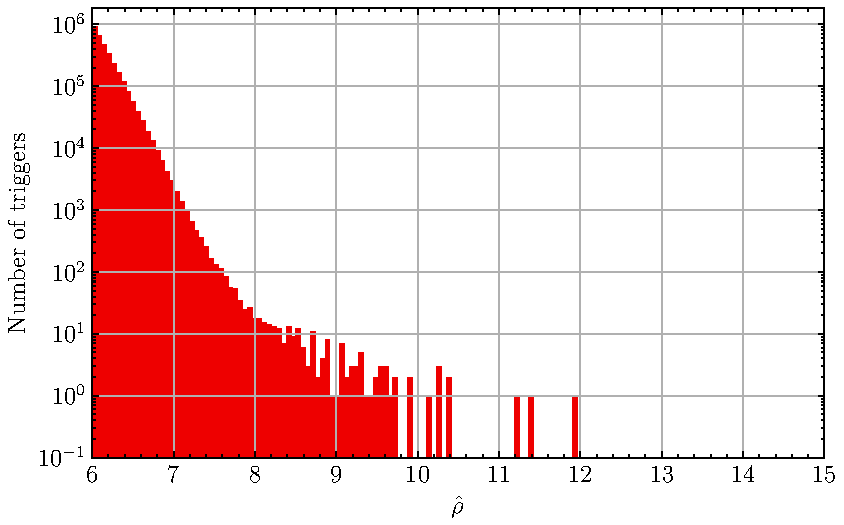
\includegraphics[width=1.0\linewidth]{images/5_pycbclive/plots/H1-newsnr_trigs.pdf}
    \caption{The new-SNR, $\hat{\rho}$, distribution of LIGO-Hanford triggers for a chunk of data searched through using PyCBC Offline in the third observing run. The higher SNR triggers can be attributed to non-Gaussian noise transients. $\hat{\rho}$ has been calculated using the Allen-$\chi^{2}$~\cite{Allen_Chi:2005} and sine-Gaussian $\chi^{2}$~\cite{PyCBC_sg:2018} to re-weight SNR.}
    \label{5:fig:H1_long_tails}
\end{figure}
%
This noise falloff has historically been assumed to be gaussian in the PyCBC Live search and all templates are treated equally. There are a number of very common glitches that occur frequently in the data that can match more closely to some templates in the template bank and not others. An example of this is blip glitches~\cite{blips:2019} which resemble the \gwadj signals of high mass binary black hole mergers, therefore the templates which describe these signals will trigger more regularly on these glitches with higher $\hat{\rho}$ compared to other templates in the bank which do not look similar to any glitch class. Not only will the noise falloff no longer be Gaussian, each template is treated equally where some trigger far more frequently with higher $\hat{\rho}$.

% Introduce the noise falloff model itself
Single detector triggers found by PyCBC searches are only saved if the $\rho > 4.5$. All triggers above the threshold form the noise distribution we want to model. The noise falloff is modelled in PyCBC by taking all the triggers produced by a template and fitting an exponential function to the slope of the falloff giving the exponential fit factor, $\alpha$, and the count of triggers found with $\hat{\rho} > 6.0$, $\mu$. This process is commonly called `template fitting' and the output parameters are called the `template fits'.

PyCBC Offline searches through pre-defined chunks of IGWN data~\cite{gwtc3:2023}, which are all around one calendar week long. The search will matched filter the template bank and the data in one of these chunks and all triggers above the previously mentioned $\rho$ threshold for each template are collected and saved. These triggers are then used to calculate $\alpha$ and $\mu$ for each template and these parameters are saved to data files which contain all of the template fits for the entire template bank for that chunk of data.
%
% Figure for the template fits
% 
To understand how the template fits contributes to the ranking statistic we must first construct the ranking statistic which includes the exponential noise model. We previously defined a general detection statistic in equation~\ref{5:eqn:general-detection-statistic} which was constructed to obtain the quadrature sum statistic for a detector with stationary, Gaussian noise. This ranking statistic models the noise falloff in the distribution as a Gaussian. The new exponential fit to the noise falloff doesn't make this assumption so we return to,
%
\begin{equation}
    \Lambda(\Vec{\theta}) = \mu_{s} \frac{p^{S}(\Vec{\theta})}{p^{N}(\Vec{\theta})} ,
    \label{5:eqn:optimal-detection-statistic}
\end{equation}
where $\mu_{s}$ is the astrophysical signal rate and is assumed to be constant, $p^{S}(\Vec{\theta})$ is the signal event rate density (signal rate) and $p^{N}(\Vec{\theta})$ is the noise event rate density (noise rate). Due to expected values of signal and noise rate spanning many orders of magnitude we take the logarithm of equation~\ref{5:eqn:optimal-detection-statistic},
%
\begin{equation}
    R = \log \Lambda = \log p^{S}(\Vec{\theta}) - \log p^{N}(\Vec{\theta}).
    \label{5:eqn:signal-minus-noise-rate}
\end{equation}
The noise rate is a combination of the single detector noise rates,
%
\begin{equation}
    p^{N}(\Vec{\theta}) = A_{N} \prod_{d} r_{d}(\hat{\rho})_{d} ,
\label{5:eqn:comb-noise-rate}
\end{equation}
%
where $A_{N}$ is the `allowed area' for coincident noise events from two detectors, $A_{N\{12\}} = 2\tau_{12}$, where $\tau_{12}$ is the \gwadj travel time window between detectors $1$ \& $2$ with a small allowance for timing error (currently $0.03$ seconds) and $r_{d}$ is the single detector noise event rate density for each detector $d$. The natural logarithm of this noise rate is taken to get the final combined log noise rate,
%
\begin{equation}
    \log(p^{N}(\Vec{\theta})) = \log(A_{N}) +  \sum_{d} \log(r_{d}(\hat{\rho}_{d})) .
\label{5:eqn:comb-log-noise-rate}
\end{equation}
%
The single detector noise rate is calculated with the product of the count of triggers above the $\hat{\rho} > 6.0$, $\mu$, and the probability of $\hat{\rho}$ given the template (including $\alpha$ and $\mu$) and noise,
%
\begin{equation}
    r_{d}(\hat{\rho}_{d}; {\Vec{\theta}}; N) = \mu(\Vec{\theta}) p(\hat{\rho} | \Vec{\theta}, N) ,
\label{5:eqn:single-noise-rate}
\end{equation}
%
where
%
\begin{equation}
    p(\hat{\rho} | \Vec{\theta}, N) = \alpha(\Vec{\theta}) \exp\left(-\alpha(\Vec{\theta})\cdot\left(\hat{\rho} - \hat{\rho}_{thresh}\right)\right)
\label{5:eqn:p-definition}
\end{equation}
%
thereby giving the single detector noise rate as,
%
\begin{equation}
    r_{d}(\hat{\rho}; {\Vec{\theta}}, N) = \mu(\Vec{\theta}) \alpha(\Vec{\theta}) \exp\left(-\alpha(\Vec{\theta}) \cdot (\hat{\rho} - \hat{\rho}_{thresh})\right)
\label{5:eqn:single-noise-rate-full}
\end{equation}
%
and when the natural logarithm is taken we arrive at the complete single detector log noise rate,
%
\begin{equation}
    \log r_{d}(\hat{\rho}) = \log\mu(\Vec{\theta}) +  \log\alpha(\Vec{\theta}) - \alpha(\Vec{\theta}) \cdot(\hat{\rho} - \hat{\rho}_{thresh})
\label{5:eqn:single-log-noise-rate}
\end{equation}
%
for each detector, $d$.

\section{\label{5:sec:injection-tests}Measuring improvements in search sensitivity}

% Motivation for investigating the sensitivity increase
% How do we quantify sensitivity
To quantifiably demonstrate that the new additions to the ranking statistic have improved the live search we can investigate the differences in sensitivity when the PSD variation and exponential noise model are included. We quantify the sensitivity of the search by calculating the sensitive volume in which we can observe \gwadj signals. The sensitive volume is calculated by measuring the detection efficiency of different distance bins that are taken from an injection set and then multiplying by the volume enclosed by the distance bins. The volume of each bin is then summed to find the total sensitive volume of the search~\cite{rw_snr_eq:2012}.

We can search through a period of data which contains an injection set with two instances of the PyCBC Live search, one containing the new ranking statistic additions and one representing the original ranking statistic. The ratio of the new statistic sensitive volume to the original statistic sensitive volume will indicate the change in sensitivity when including the new ranking statistic components.

% What is the injection set
We have chosen to test the ranking statistic changes to PyCBC Live using a smaller template bank than the current PyCBC Live template bank, which contains over $730,000$ templates~\cite{PyCBC_Live:2018}. PyCBC-BBH is a search focussed on binary black hole (BBH) signals performed in the third observing run~\cite{gwtc3:2023, PyCBC_focussed_bbh:2024} and used a template bank with only $15,436$ templates with the drawback that we are only considering BBH signals. This smaller template bank uses fewer computational resources and allows a full week of data to be searched through with PyCBC Live in as little as $1$ day. The injection sets used in the third observing run is shown in table~\ref{5:tab:injection-set}~\cite{gwtc3:2023} with rows for the specific cuts on injections for both the PyCBC-broad (full parameter space search) and PyCBC-BBH search.
% % ORIGINAL TABLE FROM THE PAPER, I'VE REMOVE SOME THINGS
% \begin{table}[]
%     \centering
%     \begin{tabular}{c c cccccc }
%         \multicolumn{2}{c}{ } & Mass & Mass &  Spin & Spin & Redshift & Maximum  \\
%         \multicolumn{2}{c}{ } & distribution & range ($M_{\odot}$) & range & orientations & evolution & redshift  \\
%         \hline
%         \multirow{6}{*}{{Injections}} & \multirow{2}{*}{BBH} &  $\left.p(m_{1}) \propto m_{1}{}^{-2.35}\right.$ \rule{0pt}{1.05\normalbaselineskip} & $2 < m_{1} < 100$ & \multirow{2}{*}{$\left|\chi_{1,2}\right| < 0.998$} & \multirow{2}{*}{Isotropic} & $ \multirow{2}{*}{$\kappa = 1$}$ & \multirow{2}{*}{$1.9$}  \\
%          & & $p(m_{2}|m_{1}) \propto m_{2}$ & $2 < m_{2} < 100$ & & & & \\[0.05\normalbaselineskip]
%          & \multirow{2}{*}{NSBH} & $\left.p(m_{1}) \propto m_{1}^{-2.35}\right.$ & $2.5 < m_{1} < 60$ & $\left|\chi_1\right| < 0.998$ & \multirow{2}{*}{Isotropic} & $ \multirow{2}{*}{$\kappa = 0$}$ &  \multirow{2}{*}{$0.25$} \\
%          & & Uniform & $1 < m_{2} < 2.5$ & $\left|\chi_2\right| < 0.4$ & & &  \\[0.05\normalbaselineskip]
%          & \multirow{2}{*}{BNS} & \multirow{2}{*}{Uniform} & $1 < m_{1} < 2.5$ & \multirow{2}{*}{$\left|\chi_{1,2}\right| < 0.4$} & \multirow{2}{*}{Isotropic} & $ \multirow{2}{*}{$\kappa = 0$}$ & \multirow{2}{*}{$0.15$}  \\
%          & & & $1 < m_{2} < 2.5$ & & & & \\%[0.25\normalbaselineskip]
%         \hline
%         \multirow{3}{*}{PyCBC-broad $p_{astro}$} & BBH & & $\mathcal{M} > 4.353 $ & & & & \\[0.05\normalbaselineskip]
%         & NSBH & & \hspace{-1.25cm} $ 2.176 < \mathcal{M} < 4.353 $ & & & & \\[0.05\normalbaselineskip]
%         & BNS & & $ \mathcal{M} < 2.176 $ & & & & \\%[0.25\normalbaselineskip]
%         \hline
%         {PyCBC-BBH $p_{astro}$} & {BBH} & & $\mathcal{M} > 4.353 $ & & & \\
%     \end{tabular}
% \end{table}
% %
%
\begin{table}[ht]
    \centering
    \begin{tabular}{c c ccc }
        \multicolumn{2}{c}{ } & Mass & Mass &  Spin \\
        \multicolumn{2}{c}{ } & distribution & range ($M_{\odot}$) & range  \\
        \hline
        \multirow{6}{*}{{Injections}} & \multirow{2}{*}{BBH} &  $\left.p(m_{1}) \propto m_{1}{}^{-2.35}\right.$ \rule{0pt}{1.05\normalbaselineskip} & $2 < m_{1} < 100$ & \multirow{2}{*}{$\left|\chi_{1,2}\right| < 0.998$} \\
         & & $p(m_{2}|m_{1}) \propto m_{2}$ & $2 < m_{2} < 100$ & \\[0.05\normalbaselineskip]
         & \multirow{2}{*}{NSBH} & $\left.p(m_{1}) \propto m_{1}^{-2.35}\right.$ & $2.5 < m_{1} < 60$ & $\left|\chi_1\right| < 0.998$ \\
         & & Uniform & $1 < m_{2} < 2.5$ & $\left|\chi_2\right| < 0.4$  \\[0.05\normalbaselineskip]
         & \multirow{2}{*}{BNS} & \multirow{2}{*}{Uniform} & $1 < m_{1} < 2.5$ & \multirow{2}{*}{$\left|\chi_{1,2}\right| < 0.4$} \\
         & & & $1 < m_{2} < 2.5$ & \\%[0.25\normalbaselineskip]
        \hline
        \multirow{3}{*}{PyCBC-broad} & BBH & & $\mathcal{M} > 4.353 $ & \\[0.05\normalbaselineskip]
        & NSBH & & \hspace{-1.25cm} $ 2.176 < \mathcal{M} < 4.353 $ & \\[0.05\normalbaselineskip]
        & BNS & & $ \mathcal{M} < 2.176 $ & \\%[0.25\normalbaselineskip]
        \hline
        {PyCBC-BBH} & {BBH} & & $\mathcal{M} > 4.353 $ \\
    \end{tabular}
    \caption{Recreated from~\cite{gwtc3:2023}. The intrinsic parameter distributions used to generate the injection set used for computing the sensitive volume change when including the PSD variation statistic and exponential noise model. Here PyCBC-broad is the PyCBC offline search across the full template bank and parameter space, including templates representing binary black hole, neutron star black hole and binary neutron star signals. This is comparable to the template bank used by the PyCBC Live full-bandwidth search. PyCBC-BBH considers only templates with chirp mass, $\mathcal{M}$, greater than $4.353 M_{\odot}$ which includes only binary black hole signals. This is the same template bank that is used for the analysis in this chapter.}
    \label{5:tab:injection-set}
\end{table}
%
%
% DESCRIBE WHY THE TEST IS STILL REPRESENTATIVE JUST USING THE BBH INJECTIONS

% How did we test the search changes
As previously mentioned, the template fits are measured from the triggers found in the previous week to the week currently being searched through. Therefore to perform our injection set test we need to do an initial search with PyCBC Live using the original ranking statistic to generate a week's worth of triggers and create template fit statistics. The second week of data is then created containing a large number of injected \gwadj signals that is searched through with PyCBC Live using both the original ranking statistic and the new ranking statistic. The two weeks of O3b \gwadj data used lasted from 06 January 2020 23:59:42 to 20 January 2020 23:59:42 and, according to the \gwadj catalogue for the third observing run~\cite{gwtc3:2023}, there are no known \gwadj signals present. After both searches have completed analysing the second week of data we can estimate the sensitivity improvement. We can choose a threshold false-alarm rate (FAR) and count the number of injections in both searches that have been found with a FAR lower than that number, if the counted number of injections is higher when including the new ranking statistic additions we have seen an increase in the sensitivity of the search. We can do this for a range of FAR values from $10^{4} - 10^{-4}$ to build up a picture of the sensitivity ratio curve.

\section{\label{5:sec:sensitivity-improvements}Improvements in sensitivity}

By adding the PSD variation and the exponential noise model to the ranking statistic we expect to find \gwadj injections with a greater significance than before. This significance is determined by the FAR of the injection, which has a direct mapping to the ranking statistic value, an event found with a FAR of $1$ per year would indicate that an event with the exact same parameters is expected to be seen in the data caused by non-astrophysical noise-not a real event-once per year of analysis time. We commonly use the inverse false-alarm rate (IFAR) with units of $years$ where a large IFAR indicates a more confident detection. An IFAR threshold is chosen to separate events which are real from those that are false alarms. A balance must be made to avoid contaminating the detection catalogue with a large number of potential false alarms while not missing any real events. In this analysis we are considering only two detectors, allowing potentially more false-alarms from coincident noise when compared to a three detector configuration and therefore we have chosen a more conservative IFAR threshold of $1$ year to assess sensitivity improvements. The current threshold for LIGO/Virgo alert generation is $1$ per $2$ months~\cite{PyCBC_Live:2018} so low-latency \gwadj searches will identify more \gwadj events but these detections have additional post detection checks from data quality checks from detector characterisation~\cite{O2O3_DetChar:2021} and parameter estimation~\cite{gwtc3:2023} which can also rule out false-alarms and to prevent catalogue contamination.

% This is a low latency search so a threshold is hard to determine concretely.

% How do we compare sensitivity of the two searches using the significance of the injections
To measure the sensitivity improvement of the new ranking statistic we count the number of injections found by both searches over a range of IFAR values from $10^{-4} - 10^{4}$ and take the ratio of the counts. The injection set is pre-weighted to ensure each injection represents an equal volume, therefore instead distance binning, as described in section~\ref{5:sec:injection-tests}, we can simply count the number of injections seen by each search.
% Sensitivity Increase Plot
%
\begin{figure}
  \centering
  \begin{minipage}[t]{1.0\linewidth}
  
    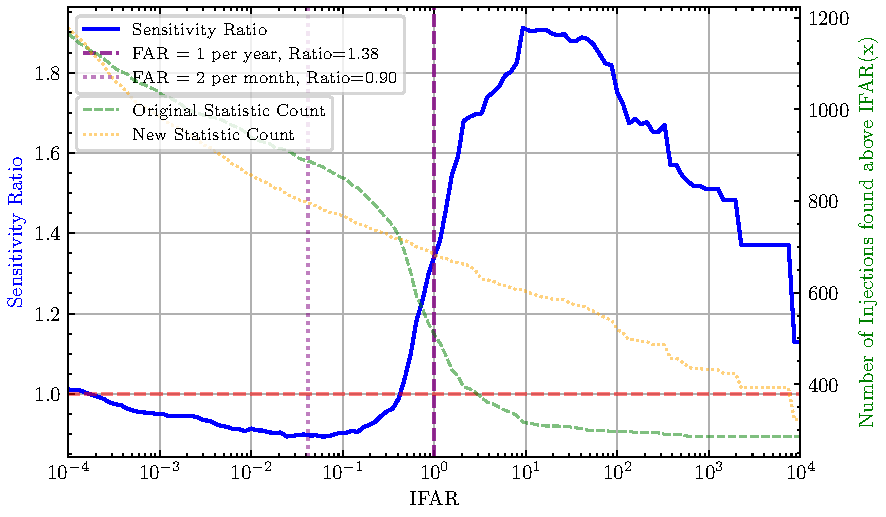
\includegraphics[width=1.0\textwidth]{images/5_pycbclive/plots/fits_psd_vt_ratio_with_counts.pdf}
    \caption{The sensitive volume ratio between a PyCBC Live search whose ranking statistic contains PSD variation and an exponential noise model and a PyCBC Live search using the original ranking statistic used by PyCBC Live during the third observing run as a function of inverse false-alarm rate (IFAR). The blue curve represents the sensitivity ratio computed by comparing the number of injections detected with an IFAR exceeding the corresponding x-axis value. An increase in sensitivity is indicated by values greater than 1, the horizontal red-dashed line. Two vertical dashed lines at fixed false-alarm rates (FAR) highlight specific thresholds: FAR = 1 per year (dark purple, dashed) with a sensitivity ratio of 1.38, and FAR = 2 per month (light purple, dotted) with a sensitivity ratio of 0.90. The green and orange curves represent the cumulative number of injections detected in the old and new searches, respectively, as a function of IFAR.}
    \label{5:fig:fits-psdvar-sensitivity}

  \end{minipage}
\end{figure}
%
% Comments about the weird shape of the plot
Figure~\ref{5:fig:fits-psdvar-sensitivity} shows the sensitivity ratio plot comparing the new statistic search to the original statistic search. We see $35\%$ more injections with an IFAR greater than our threshold of $1$ year which is a very large increase in sensitivity however at a FAR of $2$ per month we see a sensitivity decrease of $10\%$. To understand the shape of the sensitivity curve we can look at the new additions to the ranking statistic and understand further how they are changing the significance of individual injections.

\section{\label{5:sec:injection-investigations}Changes in injection significance}

% How do we map from Ranking Stat to FAR??

% How do IFAR and Significance relate
\begin{figure}
      \centering
    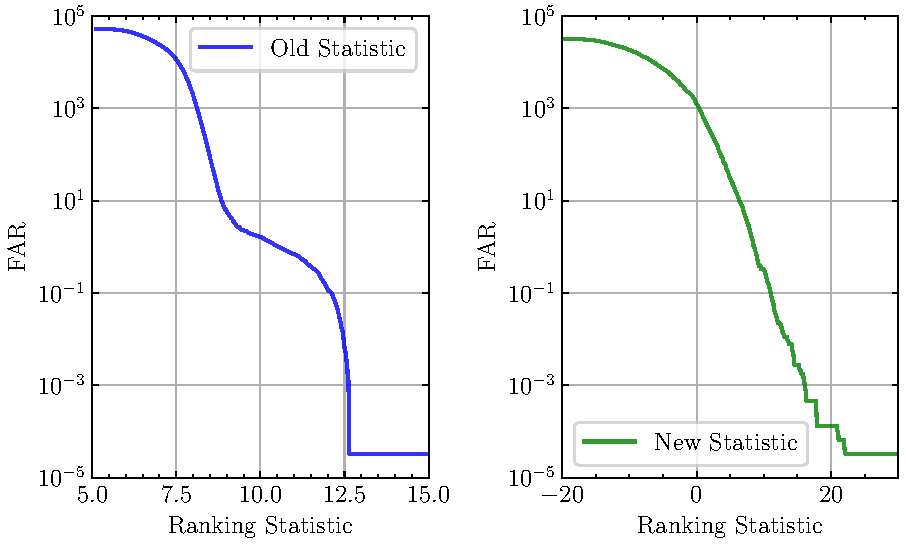
\includegraphics[width=1.0\textwidth]{images/5_pycbclive/plots/fits_psd_far_vs_stat.pdf}
    \caption{The mapping between false-alarm rate (FAR) and ranking statistic for the original PyCBC Live ranking statistic used in the third observing run (left, blue) and the new PyCBC Live ranking statistic including PSD variation and an exponential noise model (right, green). Ranking statistic values cannot be compared between ranking statistics but injection FARs can be. Higher ranking statistic values indicate better, lower FARs. The original ranking statistic has a narrower range of allowed ranking statistic values ($5 - 12.5$) along with a distinct curvature whereas the new statistic ranking statistic can take a broader range of ranking statistic values ($-20-22$) and has a relatively smooth drop off with increasing ranking statistic values.}
    \label{5:fig:fits-psdvar-far-stat}
\end{figure}
%
The ranking statistic assigned to each event can be mapped directly to FAR, shown in figure~\ref{5:fig:fits-psdvar-far-stat}. Changing the ranking statistic calculation will lead to incomparable values between searches but the individual injection IFAR values can be compared. The PyCBC Live search will matched filter the template bank and the data and where the resulting $\rho$ and $\hat{\rho}$ is above pre-defined thresholds (both $4.5$ in the third observing run) the trigger is kept. The coincidence ranking statistic value is calculated and then a ranking statistic value is assigned to the event. The initial $\rho$ values are the same between the two searches because these depend only on template and data but $\hat{\rho}$ depends on the single detector ranking statistic which has the addition of PSD variation in our new statistic, therefore it is possible for the PSD variation to prevent the saving of a trigger due to a trigger's $\hat{\rho}$ being re-weighted below the threshold.

% How does the new statistic change the injections found
We can plot the IFAR value of each injection that has been found in both searches, seen in 
figure~\ref{5:fig:ifar-ifar-fits-psdvar-shaded}.
%
\begin{figure}
      \centering
    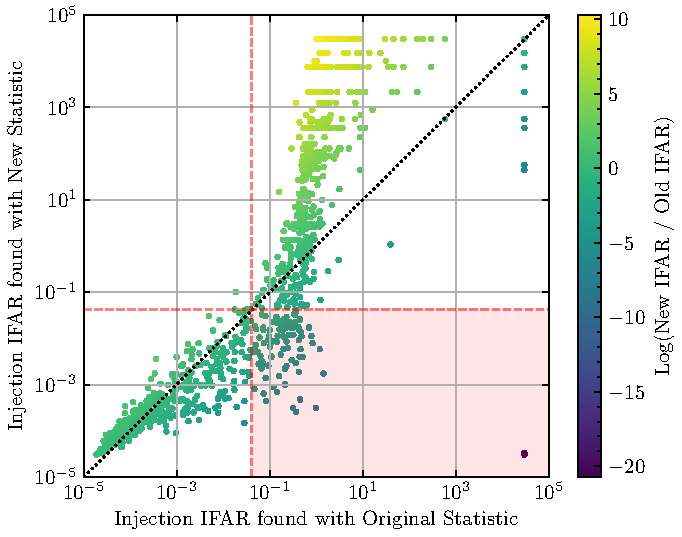
\includegraphics[width=1.0\textwidth]{images/5_pycbclive/plots/fits_psd_ifar_vs_ifar_shaded_region.pdf}
    \caption{The inverse false-alarm rate (IFAR) values recorded for each injection that was seen by both the PyCBC Live search that includes the PSD variation and exponential noise model in the ranking statistic and the PyCBC Live search using the same ranking statistic as used in the third observing run. Each point represents an injection from the injection set, with the x-axis showing the IFAR recorded using the original ranking statistic and the y-axis showing the IFAR recorded using the new ranking statistic. The color bar indicates the logarithmic difference in IFAR between the two searches, with positive values (yellow) indicating better performance of the new statistic and negative values (purple) indicating a worse performance with the new statistic. The dashed line at y=x represents equal IFAR values for both searches. The vertical and horizontal red dashed lines denote a false-alarm rate threshold of $2$ per month. The highlighted region in the bottom right of the plot indicates excess injections that have been seen by the original ranking statistic above the $2$ per month threshold and by the new ranking statistic below the $2$ per month threshold.}
    \label{5:fig:ifar-ifar-fits-psdvar-shaded}
\end{figure}
%
Within figure~\ref{5:fig:ifar-ifar-fits-psdvar-shaded} we have plotted a line on the diagonal $y=x$, injections above this line ($y > x$) have been found with a larger IFAR with the new ranking statistic and injections below ($y < x$) have been found with a lower IFAR with the new statistic. Figure~\ref{5:fig:fits-psdvar-sensitivity} highlighted the decrease in sensitivity at a FAR of $2$ per month, this decrease is due to an excess number of injections in the red-shaded box in the bottom-right of figure~\ref{5:fig:ifar-ifar-fits-psdvar-shaded}, this region represents injections which have been found by the original ranking statistic below a FAR of $2$ per month but with a FAR above $2$ per month when found by the new ranking statistic. We now proceed to explore these results, investigating why the injections found in the red-shaded box have been down-ranked and other interesting features.

\subsection{\label{5:sec:ignoring-psdvar}Effects of PSD variation on sensitivity}

The injections shown in figure~\ref{5:fig:ifar-ifar-fits-psdvar-shaded} that lie below the $y = x$ diagonal line have been found with a lower significance when including the PSD variation and the exponential noise model in the ranking statistic. We can separate the new additions and investigate the individual contributions to the changes in sensitivity.

The PSD variation statistic measures the non-stationary noise in the data and applies a weighting to the trigger $\rho$ value calculated by the matched filter of template and data, prior to the calculation of $\hat{\rho}$. To understand the effect of the PSD variation statistic on the injection significance we can compare the IFAR of injections found by the new statistic which includes both the PSD variation statistic and the exponential noise model and the IFAR of the same injections but with only the addition of the exponential noise model. This comparison is shown in figure~\ref{5:fig:ifar-ifar-fits-vs-fits-psdvar}
%
\begin{figure}
       \centering
    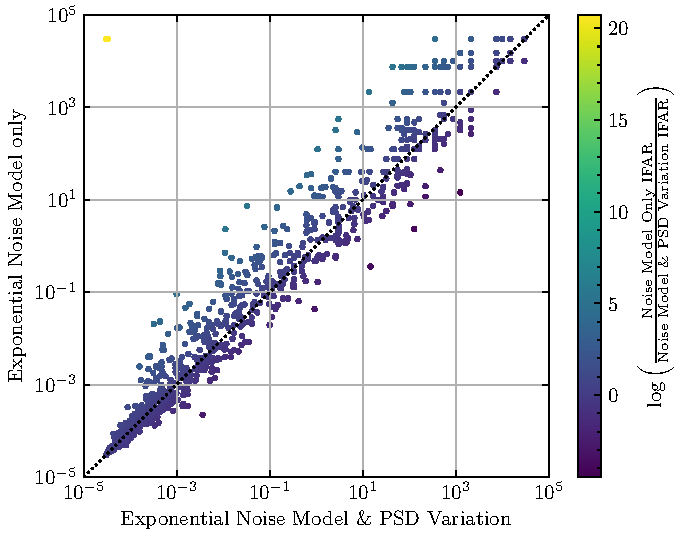
\includegraphics[width=1\textwidth]{images/5_pycbclive/plots/fits_only_fits_psd_var_ifar_vs_ifar.pdf}
    \caption{The inverse false-alarm rate (IFAR) values recorded for injections that were seen by both the PyCBC Live search that includes new additions of the PSD variation statistic and exponential noise model in the ranking statistic and the PyCBC Live search which has new additions of only the exponential noise model. Each point represents an injection from the injection set, with the x-axis showing the IFAR recorded by the PyCBC Live search including the exponential noise model and PSD variation ranking statistic and the y-axis showing the IFAR recorded by the PyCBC Live search which has added only the exponential noise model. The color bar indicates the logarithmic difference in IFAR between the two searches, with positive values (yellow) indicating better performance when \textbf{not} including PSD variation and negative values (purple) indicating a better performance with the PSD variation statistic. The dashed line at y=x represents equal IFAR values for both searches.}
    \label{5:fig:ifar-ifar-fits-vs-fits-psdvar}
\end{figure}
%
In this comparison, $550$ injections were found with a higher significance when \textbf{not} including PSD variation, $399$ were found with a higher IFAR when including PSD variation and $326$ were found with the same IFAR. We can also observe a greater dispersion of injections found above the diagonal line when compared to those found below it, meaning injections found above the diagonal line are found with a greater significance difference than those found below the line. Alongside this general trend we can see a few injections in the top-left of the plot which have had a very large increase in significance when we do not include PSD variation in the statistic, these injections correspond to the heavily down-ranked injections in the bottom-right of figure~\ref{5:fig:ifar-ifar-fits-psdvar-shaded}.

% Talk about sensitivity difference
We can compare the sensitivity change when including the PSD variation statistic by plotting the sensitivity curve in figure~\ref{5:fig:vt-ratio-f-fo}.
%
\begin{figure}
       \centering
    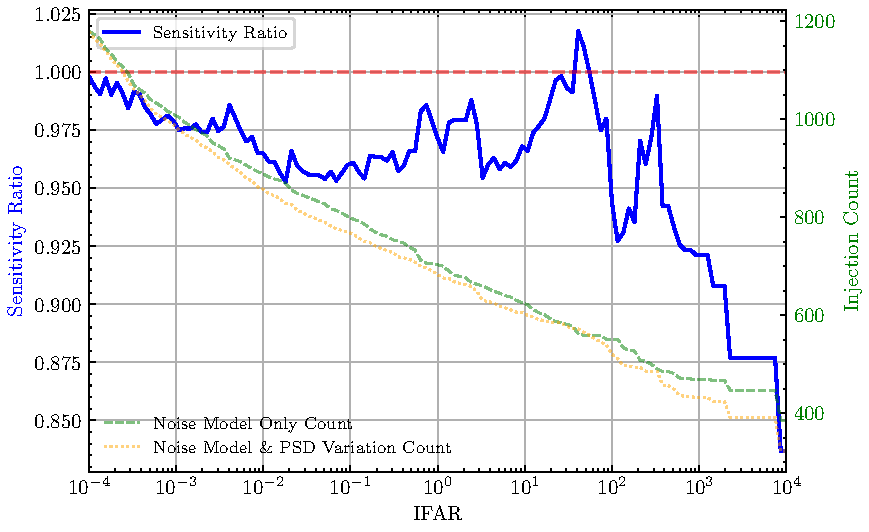
\includegraphics[width=1.0\textwidth]{images/5_pycbclive/plots/fits_only_fits_psd_vt_ratio.pdf}
    \caption{A comparison of sensitive volume ratio between two PyCBC Live searches: one which includes the addition of the PSD variation statistic and an exponential noise model in the ranking statistic and one which includes only the addition of the exponential noise model. The blue curve represents the sensitivity ratio computed by comparing the number of injections detected with an inverse false-alarm rate (IFAR) exceeding the corresponding x-axis value. An increase in sensitivity is indicated by values greater than 1, the horizontal red-dashed line. The green dashed curve represents the cumulative number of injections detected as a function of IFAR by the PyCBC Live search with added PSD variation and the exponential noise model. The orange dashed curve represents the cumulative number of injections detected as a function of IFAR by the PyCBC Live search with only the exponential noise model added.}
    \label{5:fig:vt-ratio-f-fo}
\end{figure}
%
From this is it clear to see there is a small decrease in sensitivity when including the PSD variation statistic in the new ranking statistic. We note that the current implementation of PSD variation in PyCBC Offline has problems, specifically, PSD variation is eliminating extremely significant low-mass injections. Investigation into the PSD variation issues is being conducted and future iterations of PSD variation may improve its performance in PyCBC Live.

We have previously described how the PyCBC Live search re-calculates the PSD every analysis segment and replaces the currently used PSD when the BNS distance of the new PSD differs from the current PSD's by more than $1\%$. This reduces the need to include the PSD variation statistic to tackle non-stationary noise in the data. In light of the sensitivity decrease when including PSD variation we make the choice to not use PSD variation in the ranking statistic going forward.

% Noise model only sensitivity
When adding only the exponential noise model to the ranking statistic we can re-analyse the sensitivity improvements to produce figure~\ref{5:fig:vt-ratio-fits-only}.
%
\begin{figure}
       \centering
    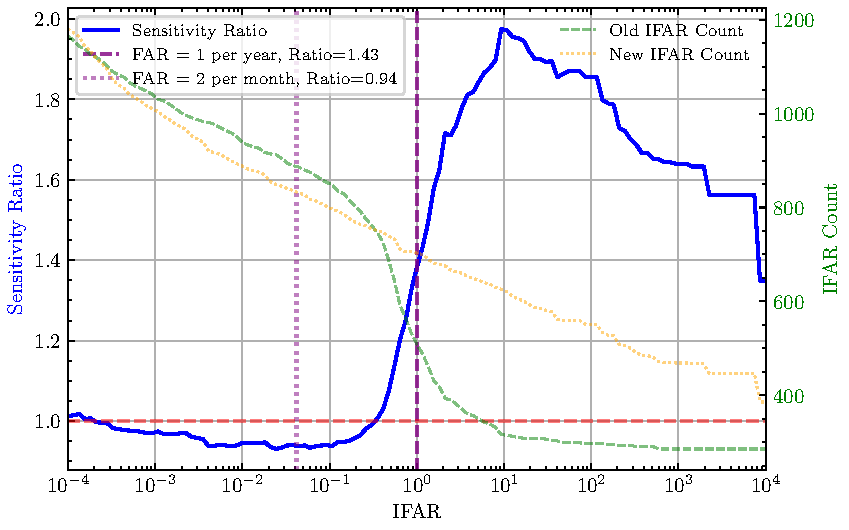
\includegraphics[width=1.0\textwidth]{images/5_pycbclive/plots/fits_only_vt_ratio_with_counts.pdf}
    \caption{A comparison of sensitive volume ratio between a PyCBC Live search whose ranking statistic contains an exponential noise model and a PyCBC Live search using the original ranking statistic used by PyCBC Live during the third observing run as a function of inverse false-alarm rate (IFAR). The blue curve represents the sensitivity ratio computed by comparing the number of injections detected with an IFAR exceeding the corresponding x-axis value. An increase in sensitivity is indicated by values greater than 1, the horizontal red-dashed line. Two vertical dashed lines at fixed false-alarm rates (FAR) highlight specific thresholds: FAR = 1 per year (dark purple, dashed) with a sensitivity ratio of 1.43, and FAR = 2 per month (light purple, dotted) with a sensitivity ratio of 0.94. The green and orange curves represent the cumulative number of injections detected in the old and new searches, respectively, as a function of IFAR.}
    \label{5:fig:vt-ratio-fits-only}
\end{figure}
%
This shows a greater increase across the IFAR range, with sensitivity increase at a FAR of $1$ per year of $43\%$ and a decrease of $6\%$ at a FAR of $2$ per month.

% Noise model only IFAR vs IFAR with regions
We can plot the IFAR vs IFAR plot for the search including only the exponential noise model in the ranking statistic compared to the original search, seen in figure~\ref{5:fig:ifar-ifar-fits-only-regions}, and when we compared to figure~\ref{5:fig:ifar-ifar-fits-psdvar-shaded} we can see that the distribution of injections at low IFARs has decreased in dispersion around the diagonal line.
% 
\begin{figure}
       \centering
    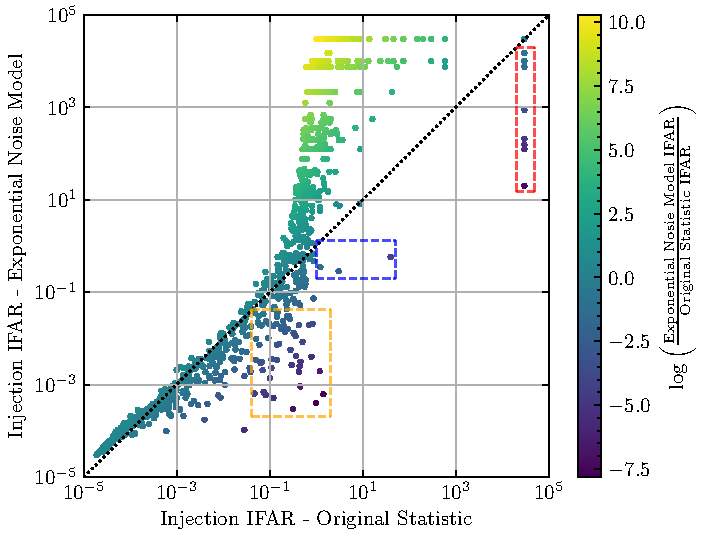
\includegraphics[width=1.0\textwidth]{images/5_pycbclive/plots/fits_only_ifar_vs_ifar_regions.pdf}
    \caption{The inverse false-alarm rate (IFAR) values recorded for each injection that was seen by both the PyCBC Live search that includes the exponential noise model in the ranking statistic and the PyCBC Live search using the same ranking statistic used in the third observing run. Each point represents an injection from the injection set, with the x-axis showing the IFAR recorded using the original ranking statistic and the y-axis showing the IFAR recorded using the exponential noise model ranking statistic. The color bar indicates the logarithmic difference in IFAR between the two searches, with positive values (yellow) indicating better performance when including the exponential noise model in the statistic and negative values (purple) indicating a better performance with the original statistic. The dashed line at y=x represents equal IFAR values for both searches. Three regions containing injections that have been down-ranked and will be investigated have been highlighted in dashed boxes.}
    \label{5:fig:ifar-ifar-fits-only-regions}
\end{figure}
%
We have highlighted three regions of interest which contains injections that have decreased in significance that we will investigate further and understand the cause of their down-ranking.

\subsection{\label{5:sec:poor-temp-fits}Templates which trigger frequently with large SNRs}

% Log(noise rate) equation
% Combined log(noise rate) equation
% Low Alpha + High Rate == High Combined Log(noise rate)
% Plot Alpha vs Rate, colour Log(noise rate)
% Plot Alpha vs SNR, colour Log(noise rate)

% Motivation here is the separation of PSD Variation and Template Fits to see how they change the sensitivity of each injection or how the sensitivity change manifests

% What identifies a template as having a high noise rate
The new exponential noise model in the ranking statistic allows us to model individual template noise distributions depending using that template's historical triggers. This allows us to down-rank templates which frequently trigger on non-Gaussian noise with a high $\hat{\rho}$. As describe in equation~\ref{5:eqn:comb-noise-rate}, the exponential noise model is characterised by an exponential fit to the slope of the trigger distribution and is quantified by the exponential fit factor, $\alpha$, and the count of triggers above $\hat{\rho}_{thresh}$, $\mu$. Therefore, using these two parameters we must be able to differentiate between templates which trigger frequently on noise with large $\hat{\rho}$ and those that rarely trigger on noise. All templates in the bank will trigger on both Gaussian noise and glitches in our data, and after applying all signal consistency tests these triggers might still might have $\hat{\rho} > 8.0$. 

Figure~\ref{5:fig:template-fits} shows an example of the exponential fitting to a group of template's noise distributions to obtain the exponential fit factors. This group of templates have effective spin, $\chi_{eff} = -0.333 - 0.333$, symmetric mass ratio $\eta = 0.208 - 0.229$ and the different template duration bins and corresponding exponential fitting factors have been plotted over the top.
%
\begin{figure}
    \centering
    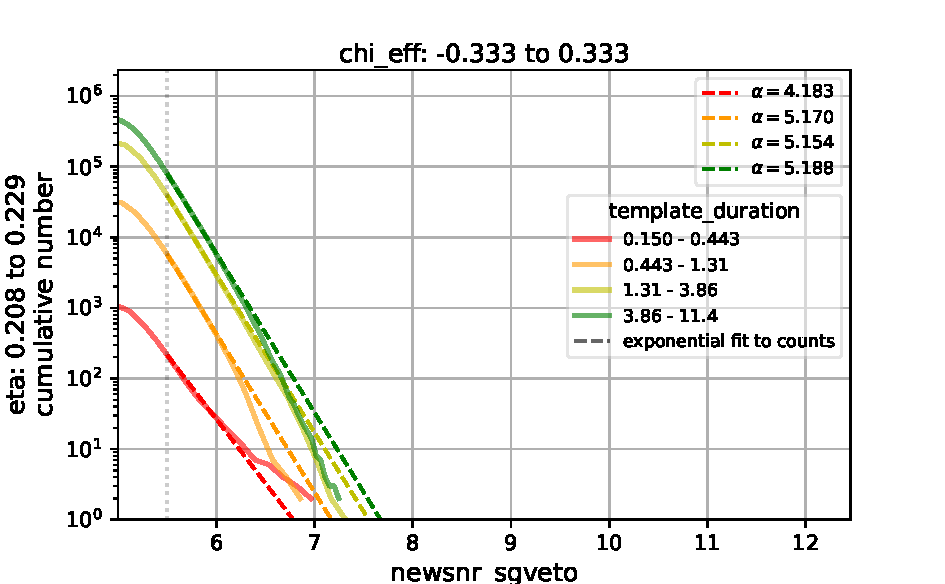
\includegraphics[width=1.0\textwidth]{images/5_pycbclive/plots/fit_plot.pdf}
    \caption{The noise distribution and template fits for a bin which contains triggers from templates which have symmetric mass ratio, $\eta$, between $0.208 - 0.229$ and effective spin, $\chi_{eff}$, between $-0.333 - 0.333$. The template triggers are further split into 4 bins depending on the duration of the template responsible for the trigger (in seconds). The solid coloured lines represent the cumulative counts of triggers that have been found in a template duration bin with $\rho$ that has been re-weighted by the traditional $\chi^{2}$~\cite{Allen_Chi:2005} and the sine-gaussian $\chi^{2}$~\cite{PyCBC_sg:2018} to obtain new signal-to-noise ratio, $\hat{\rho}$. The dashed coloured lines represent the exponential fit that has been made to the cumulative counts for each template duration bin where the exponential fit factor value, $\alpha$, is displayed in the top right most legend.}
    \label{5:fig:template-fits}
\end{figure}
%
This figure shows the difference in exponential fit slopes for the varying template bins and it can be seen that the bins which trigger more frequently with a higher new SNR have shallower slopes (lower $\alpha$) compared to the steeper slopes (higher $\alpha$) in other bins. Equation~\ref{5:eqn:single-log-noise-rate} shows that higher $\alpha$ values correspond to lower noise rates and lower $\alpha$ and higher $\mu$ values produce higher noise rates.

Templates which trigger more frequently and with a large $\hat{\rho}$ on noise will be down ranked by the ranking statistic but real \gwadj signals that match this template will also be down ranked if they have low single detector $\hat{\rho}$. We can plot equation~\ref{5:eqn:single-log-noise-rate}, which calculates the single detector noise rate, in figure~\ref{5:fig:log-noise-static-snr} to show the dependence on $\alpha$ and $\mu$. In our search $\alpha$ can take values $1.5 - 6.0$ and $\mu$ from $5 - 45$ and we have used a static $\hat{\rho}$ of $10.0$ in the equation. It can be seen that a higher $\alpha$ value has a greater effect on the noise rate and the contribution from $\mu$ has a maximum value of $3.8$, $ + \log\mu$ in equation~\ref{5:eqn:single-log-noise-rate}.
%
\begin{figure}
    \centering
    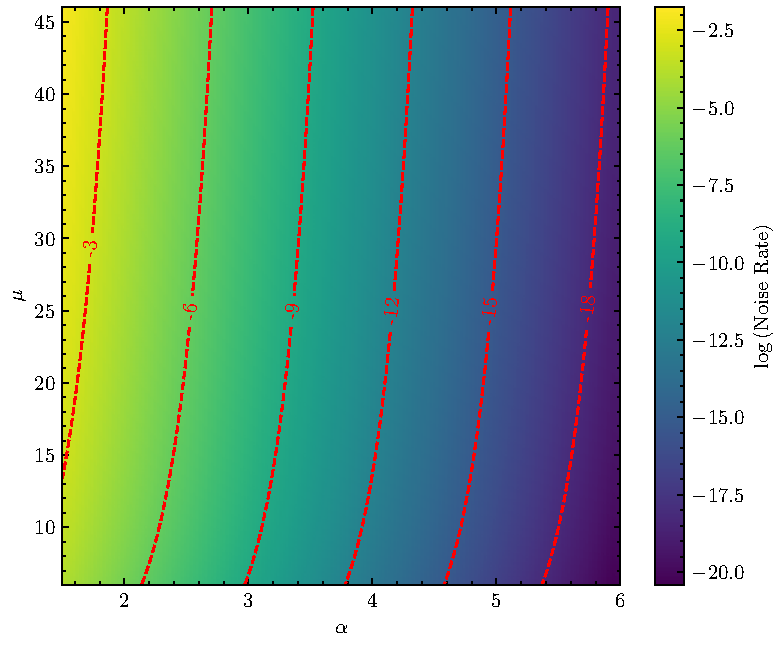
\includegraphics[width=1\textwidth]{images/5_pycbclive/plots/lognoise_alpha_rate.pdf}
    \caption{The single detector ($\log$) noise rate for varying combinations of exponential fit factor, $\alpha$, and trigger rates above a single detector statistic value ($\hat{\rho}_{thresh} = 6.0$), $\mu$. Constant contours of single detector noise rate are shown as dashed red lines, with the single detector noise rate value labelled within the contour line. This figure has been made using equation~\ref{5:eqn:single-log-noise-rate} where $\hat{\rho} = 10.0$.}
    \label{5:fig:log-noise-static-snr}
\end{figure}
%
Figure~\ref{5:fig:log-noise-static-rate} shows the noise rate's dependence on $\alpha$ and $\hat{\rho}$ while $\mu$ has been set to the benchmark noise rate of $-14.6$, which is the representative noise rate measured empirically during the second observing run. 
%
\begin{figure}
    \centering
    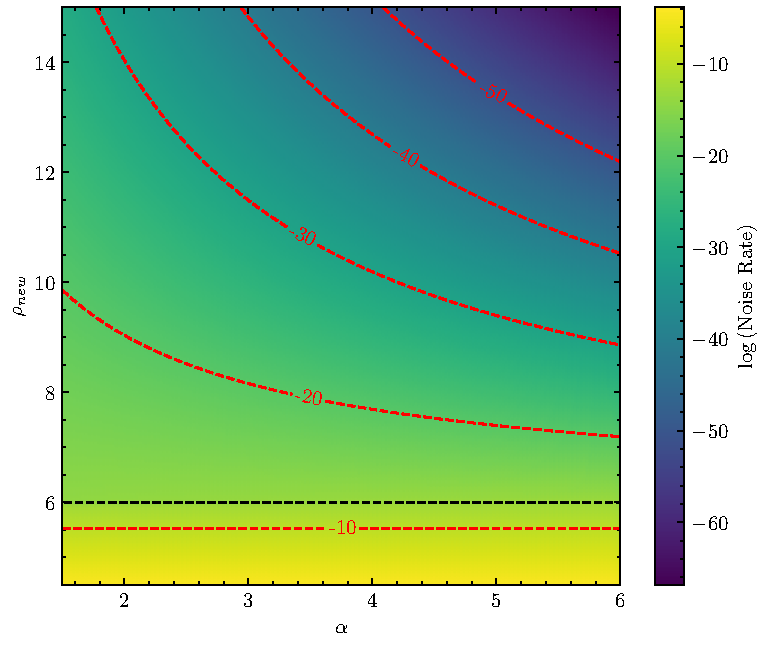
\includegraphics[width=1\textwidth]{images/5_pycbclive/plots/lognoise_alpha_snr.pdf}
    \caption{The single detector ($\log$) noise rate for varying combinations of exponential fit factor, $\alpha$, and single detector statistic value, $\hat{\rho}$. Constant contours of single detector noise rate are shown as dashed red lines, with the single detector noise rate value labelled within the contour line. This figure has been made using equation~\ref{5:eqn:single-log-noise-rate} where $\mu$ has been set equal to the benchmark noise rate $-14.6$.}
    \label{5:fig:log-noise-static-rate}
\end{figure}
%
A black dashed line has been plotted at $\hat{\rho} = 6.0$ due to triggers below this $\hat{\rho}$ threshold all being assigned $\alpha = 6.0$, therefore the noise rate below this threshold is constant for all $\alpha$ values on the plot. We can clearly see a strong correlation between $\hat{\rho}$ and noise rate with a heavy dependency on $\alpha$, to the point where high $\hat{\rho}$ triggers with low $\alpha$--while still significant--have higher noise rates than triggers with high $\alpha$.

% Plot IFAR vs IFAR, colour H1 alpha
% Plot IFAR vs IFAR, colour H1 rate
% Plot IFAR vs IFAR, colour H1 noise rate

We can plot the IFAR vs IFAR distribution for the injection set for a single detector's $\alpha$, $\mu$ and log noise rate to see if there is any clear dependence on the template fit parameters, seen in figures~\ref{5:fig:ifar-ifar-subplots}.
%
\begin{figure}
    \centering
    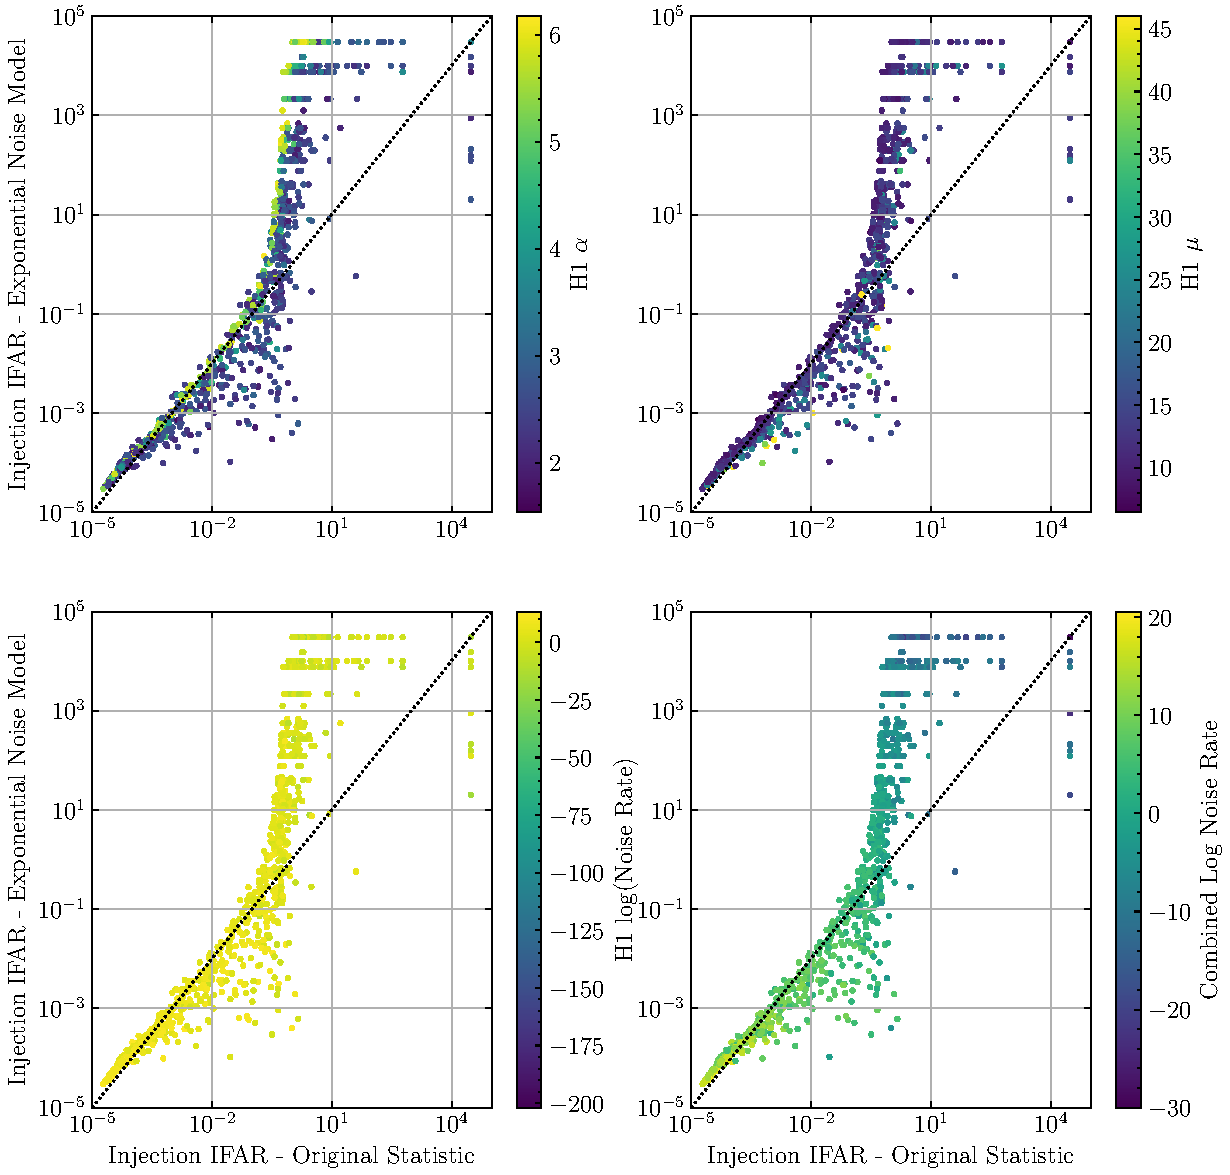
\includegraphics[width=\textwidth]{images/5_pycbclive/plots/fits_only_ifar_vs_ifar_subplots.pdf}
    \caption{The inverse false-alarm rate (IFAR) values recorded for each injection that was seen by both the PyCBC Live search that includes the exponential noise model in the ranking statistic and the PyCBC Live search using the same ranking statistic used in the third observing run. Each point represents an injection from the injection set, with the x-axis showing the IFAR recorded using the original ranking statistic and the y-axis showing the IFAR recorded using the exponential noise model ranking statistic. The top left plot is coloured by the LIGO-Hanford trigger template's exponential fit factor, $\alpha$. The top right plot is coloured by the LIGO-Hanford trigger template's count of triggers found above $\hat{\rho}_{threshold} = 6.0$, $\mu$. The bottom left plot is coloured by the LIGO-Hanford single detector ($\log$) noise rate, calculated using equation~\ref{5:eqn:single-log-noise-rate}. The bottom right plot is coloured by the combined ($\log$) noise rate, equation~\ref{5:eqn:comb-log-noise-rate}.}
    \label{5:fig:ifar-ifar-subplots}
\end{figure}
%
It is not clear from these figures that $\alpha$ (top-left) and $\mu$ (top-right) are having a large effect on the log noise shown in the bottom-left figure. There is a curve of high $\alpha$ points above the $y=x$ line in the top-left figure but no clear distinction between higher and lower $\alpha$ values corresponding to higher and lower IFAR values. As mentioned before and reinforced by the top-right plot, $\mu$ has a small effect on the noise rate and low $\mu$ values are more common than high ones.

Figure~\ref{5:fig:ifar-ifar-subplots} shows the combined detector noise rates (equation~\ref{5:eqn:comb-log-noise-rate}), where we can see a clearer distinction between high and low noise rates and how this is affecting the IFAR values. However, looking at this plot we can see that combined noise rate does not completely explain the improved significance for a number of injections, we can see clearly there are some low noise rate injections below the $y=x$ line which should have caused an increase in the significance but we have seen a decrease. Therefore we must investigate other changes to the ranking statistic.

\subsection{\label{5:sec:comparing-statistic-construction}Ranking statistic construction}

% Motivation
The original ranking statistic and our new ranking statistic both take contributions from the signal event rate density, $p^{S}(\Vec{\theta})$, and the noise event rate density, $p^{N}(\Vec{\theta})$. The construction of these ranking statistics has been detailed in sections~\ref{5:sec:old-stat-construction} and~\ref{5:subsec:template-fits} where it can be seen they include the contributions from $p^{S}(\Vec{\theta})$ differently. For comparison, the original statistic is constructed as,
%
\begin{equation}
    R = \sqrt{\hat{\rho}^{2}_{H} + \hat{\rho}^{2}_{L} + 2\log\left(p^{S}(\Vec{\theta})\right)}
    \label{5:eqn:original-statistic-repeat}
\end{equation}
%
and the statistic including the exponential noise model is,
%
\begin{equation}
    R = \log p^{S}(\Vec{\theta}) - \log\left(A_{N}\right) + \sum_{d} \log\left(r_{d}(\hat{\rho})\right),
    \label{5:eqn:new-statistic}
\end{equation}
%
where $p^{N}(\Vec{\theta})$ has been substituted with the combined noise rate defined in equation~\ref{5:eqn:comb-log-noise-rate}.

The general detection statistic (equation~\ref{5:eqn:general-detection-statistic}) was constructed so that in stationary, Gaussian noise the ranking statistic recovers the quadrature sum ranking statistic. When including the exponential noise model we are explicitly modelling the detector noise and therefore have chosen to use the optimal detection statistic (equation~\ref{5:eqn:optimal-detection-statistic}) which is simply the ratio of signal and noise event rate densities.

Equations~\ref{5:eqn:original-statistic-repeat} and~\ref{5:eqn:new-statistic} show that the original statistic quadratically adds signal rate and noise rate whereas the new noise distribution model ranking statistic will add signal and noise rates linearlly, changing the ratio of contributions from signal rate and noise rate in the ranking statistic calculation.

One particular way the different noise rate models manifests is in the ratio of the two detector $\hat{\rho}$ values. Modelling the noise distribution falloff as Gaussian causes the ranking statistic to attempt to maximise the squared sum of the $\hat{\rho}$ values found by each detector with only the signal-consistency tests to re-weight $\rho$. Our new model adds additional weights in the form of the template fits so that if a different trigger is seen with slightly lower $\hat{\rho}$ in both detectors but the template has a lower noise rate (by having higher $\alpha$ and lower $\mu$), then it will be preferred by the noise rate model. Figure~\ref{5:fig:ifar-ifar-snr-ratio} shows the injections coloured by the SNR ratio in the new statistic search.
%
\begin{figure}
  \centering
  \begin{minipage}[t]{1.0\linewidth}
    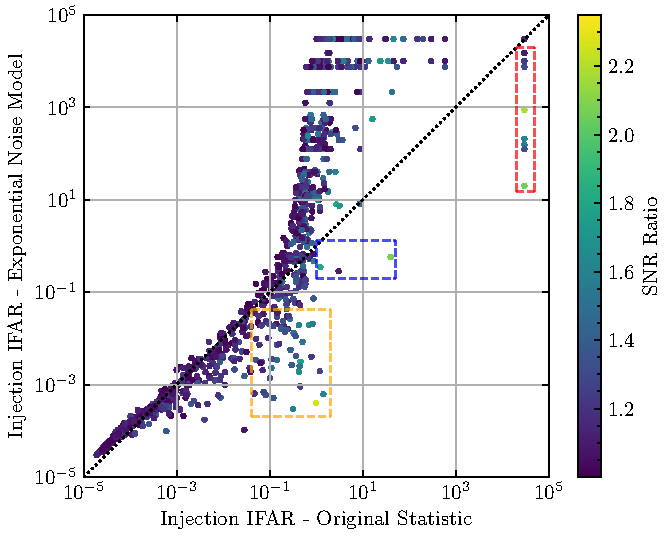
\includegraphics[width=1\textwidth]{images/5_pycbclive/plots/fits_only_ifar_vs_ifar_regions_snr_ratio.pdf}
  \end{minipage}
  \caption{The inverse false-alarm rate (IFAR) values recorded for each injection that was seen by both the PyCBC Live search that includes the exponential noise model in the ranking statistic and the PyCBC Live search using the same ranking statistic used in the third observing run. Each point represents an injection from the injection set, with the x-axis showing the IFAR recorded using the original ranking statistic and the y-axis showing the IFAR recorded using the exponential noise model ranking statistic. The injections are coloured by the SNR ratio of the two detector $\hat{\rho}$ values, set so that the SNR ratio is always greater than $1$. Three regions containing injections that will be investigated have been highlighted in dashed boxes.}
  \label{5:fig:ifar-ifar-snr-ratio}
\end{figure}
%
It can be seen that there are a number of points in regions of interest that have been down-ranked by the new search specifically because they have a high SNR ratio in the old statistic.


\subsection{\label{5:sec:diff-triggers}Different triggers selected by each search}

The ranking statistic is responsible for determining the most significant triggers in an analysis segment in the live search. As stated in equation~\ref{5:eqn:signal-minus-noise-rate} the ranking statistic is composed of two primary contributions, the signal rate and the noise rate. As described in the previous section (\ref{5:sec:comparing-statistic-construction}, both the signal and the noise rate are template dependent and therefore when the construction of the ranking statistic is changed a different template might become responsible for the preferred trigger compared with the template chosen by the original statistic search. We investigate some injections which have now been found with a different trigger when compared to the original ranking statistic search to understand how changing ranking statistic individually changes the injections.

%%% FIND SOME NEW INJECTIONS THAT HAVE BEEN FOUND WITH DIFFERENT TRIGGERS IN BOTH SEARCHES THAT HAVE SIMILAR IFAR VALUES PLEASE

Each injection in the initial injection set has an assigned index number. When a trigger is found by the search the identification number of the template responsible is saved with the trigger. Using these two values we can directly compare the template id of each injection index to find injections which have been found with with a different template id and therefore a different trigger in both searches. Table~\ref{5:tab:200-new-stat} shows an injection, with injection index $= 200$, that has been found with a different trigger in both searches.
%
\begin{table}[ht]
    \centering
    \rowcolors{2}{white}{lightgray}
    \begin{tabular}{lcc}
        \toprule
        \textbf{Injection Index = 200} & \textbf{Original Trigger} & \textbf{New Trigger} \\
        \midrule
        $\log p^{N}(\Vec{\theta})$  & -15.53 & -18.79 \\
        $\log p^{S}(\Vec{\theta})$ & -15.77 & -15.67 \\
        $R_{new}$ & -0.24 & 3.12 \\
        % IFAR & 0.00066 & 0.0067\\
        \bottomrule
    \end{tabular}
    \caption{The ($\log$) signal rate, $\log p^{S}(\Vec{\theta})$, ($\log$) noise rate, $\log p^{N}(\Vec{\theta})$, ranking statistic value, $R_{new}$ and inverse false-alarm rate (IFAR), calculated using the ranking statistic which includes an exponential noise model, for the preferred trigger found by the PyCBC Live search when using the original ranking statistic used during the third observing run (Original Trigger) and the different preferred trigger found by the PyCBC Live search using the exponential noise model ranking statistic (New Trigger) for the injection with index = 200. The ranking statistic value for both triggers is calculated from the signal rate and noise rate of the injections using equation~\ref{5:eqn:new-statistic}.}

    \label{5:tab:200-new-stat}
\end{table}
%
This table displays the values for the signal rate, $\log p^{S}(\Vec{\theta})$, the noise rate, $\log p^{N}(\Vec{\theta})$ and the ranking statistic and IFAR for both triggers calculated using the new statistic. The new trigger has a ranking statistic value of $3.12$ which makes it the preferred trigger over the trigger found using the original statistic which has a ranking statistic value of $-0.24$. This increase in ranking statistic is caused almost entirely by the lower noise rate of the new trigger and while it also has a larger signal rate this is a marginal increase. We then compare this with table~\ref{5:tab:200-old-stat} which shows the components needed to calculate the original ranking statistic value and why the original trigger was chosen over the trigger preferred by the new statistic in the original search.
%
\begin{table}[ht]
    \centering
    \rowcolors{2}{white}{lightgray}
    \begin{tabular}{lcc}
        \toprule
        \textbf{Injection Index = 200} & \textbf{Original Trigger} & \textbf{New Trigger} \\
        \midrule
        $\rho_{new, H1}$  & 15.06 & 13.50 \\
        $\rho_{new, L1}$   & 6.67 & 6.58 \\
        $\rho_{new, H1}^2 + \rho_{new, L1}^2$   & 271.29 & 225.25 \\
        $\log p^{S}(\Vec{\theta})$ & -15.77 & -15.67 \\
        $R_{old}$ & 15.48 & 13.93 \\
        % IFAR & 30174.69 & 30174.69 \\
        \bottomrule
    \end{tabular}
    \caption{The H1 new SNR, $\hat{\rho}_{H1}$, L1 new SNR, $\hat{\rho}_{L1}$, squared sum of the H1 and L1 $\hat{\rho}$s, ($\log$) signal rate, $\log p^{S}(\Vec{\theta})$, ranking statistic value, $R_{old}$, and inverse false-alarm rate (IFAR), calculated using the original ranking statistic used by PyCBC Live during the third observing run (equation~\ref{5:eqn:original-statistic}), for the preferred trigger found by the PyCBC Live search when using the original ranking statistic used during the third observing run and the different preferred trigger found by the PyCBC Live search using the exponential noise model ranking statistic for the injection with index = 200.}
    \label{5:tab:200-old-stat}
\end{table}
%
We can see that the new trigger has lower $\hat{\rho}$ in both detectors and a slightly higher signal rate. Therefore, the ranking statistic value of the original trigger is greater than that of the trigger preferred by the new ranking statistic.

We can do another analysis on the injection with index $= 445$ which was also found with different triggers in both searches. Table~\ref{5:tab:445-new-stat} shows the noise and signal rates for the injection where the noise rates are very similar but the new trigger's increase ranking statistic value is primarily due to an increase signal rate with the new trigger's template.
%
\begin{table}[ht]
    \centering
    \rowcolors{2}{white}{lightgray}
    \begin{tabular}{lcc}
        \toprule
        \textbf{Injection Index = 445} & \textbf{Original Trigger} & \textbf{New Trigger} \\
        \midrule
        $\log\left(\text{Noise Rate}\right)$  & -12.96 & -12.69 \\
        $\log\left(\text{Signal Rate}\right)$ & -4.40 & -2.74 \\
        $R_{new}$ & 8.56 & 9.95 \\
        \bottomrule
    \end{tabular}
    \caption{The ($\log$) signal rate, $\log p^{S}(\Vec{\theta})$, ($\log$) noise rate, $\log p^{N}(\Vec{\theta})$, ranking statistic value, $R_{new}$ and inverse false-alarm rate (IFAR), calculated using the ranking statistic which includes an exponential noise model, for the preferred trigger found by the PyCBC Live search when using the original ranking statistic used during the third observing run (Original Trigger) and the different preferred trigger found by the PyCBC Live search using the exponential noise model ranking statistic (New Trigger) for the injection with index = 445. The ranking statistic value for both triggers is calculated from the signal rate and noise rate of the injections using equation~\ref{5:eqn:new-statistic}.}
    \label{5:tab:445-new-stat}
\end{table}
%
Similarly, when we look at the original statistic calculation in table~\ref{5:tab:445-old-stat} we can see very similar original ranking statistic values where the signal rate increase with the new trigger is not great enough to overcome the increased $\hat{\rho}$ of the original triggers.
%
\begin{table}[ht]
    \centering
    \rowcolors{2}{white}{lightgray}
    \begin{tabular}{lcc}
        \toprule
        \textbf{Injection Index = 445} & \textbf{Original Trigger} & \textbf{New Trigger} \\
        \midrule
        $\rho_{H1,new}$  & 10.44 & 10.78 \\
        $\rho_{L1,new}$   & 8.14 & 7.16 \\
        $\rho_{H1,new}^2 + \rho_{L1,new}^2$   & 175.25 & 167.47 \\
        $\log\left(\text{Signal Rate}\right)$ & -4.40 & -2.74 \\
        $R_{old}$ & 12.90 & 12.73 \\
        \bottomrule
    \end{tabular}
    \caption{The H1 new SNR, $\hat{\rho}_{H1}$, L1 new SNR, $\hat{\rho}_{L1}$, squared sum of the H1 and L1 $\hat{\rho}$, ($\log$) signal rate, $\log p^{S}(\Vec{\theta})$, ranking statistic value, $R_{old}$, and inverse false-alarm rate (IFAR), calculated using the original ranking statistic used by PyCBC Live during the third observing run (equation~\ref{5:eqn:original-statistic}), for the preferred trigger found by the PyCBC Live search when using the original ranking statistic used during the third observing run (Original Trigger) and the different preferred trigger found by the PyCBC Live search using the exponential noise model ranking statistic (New Trigger) for the injection with index = 445.}
    \label{5:tab:445-old-stat}
\end{table}
%

The addition of the exponential noise model in the ranking statistic can explain the increase in sensitivity for some injections but others have an increase in sensitivity due to the different constructions of the ranking statistics. Different weighting has been placed on the signal and noise rates between the two searches and therefore a different trigger, with a better significance, can be chosen with a similar noise rate (the container for the exponential noise model) to the original trigger but the template associated with that trigger has a better signal rate.

\section{\label{5:sec:investigating-regions}Investigating down-ranked regions}

In sections~\ref{5:sec:ignoring-psdvar} we investigated the effect of including the PSD variation in the ranking statistic and concluded that it will not enter the ranking statistic going forward. However, when looking at the sensitivity ratio for the new ranking statistic, including only the exponential noise model, against the original statistic (figure~\ref{5:fig:vt-ratio-fits-only}) we can see that the decrease in sensitivity around at an FAR of $2$ per month is still around $6\%$.

We have discussed how changing the ranking statistic can change the significance of individual injections in sections~\ref{5:sec:poor-temp-fits}, \ref{5:sec:comparing-statistic-construction} and, \ref{5:sec:diff-triggers} and looking at the IFAR vs IFAR plot in figure~\ref{5:fig:ifar-ifar-fits-only-regions} we can highlight three region of interest which contain down-ranked injections that we must investigate and understand the reasoning behind the down-ranking. The highlighted yellow region is of particular interest as being responsible for the decrease in sensitivity at a FAR of $2$ per month.

\subsection{\label{5:sec:bottom-left-region}Injections down-ranked around FAR = 2 per month}

The sensitive volume ratio between the new ranking statistic search and the original ranking statistic search (figure~\ref{5:fig:vt-ratio-fits-only}) highlights a drop in the sensitive ratio at an approximate FAR of $2$ per month. The region responsible for this drop is highlighted on figure~\ref{5:fig:ifar-ifar-fits-only-regions} in a yellow dashed box and a zoomed in version of this figure can be seen in figure~\ref{5:fig:bottom-left-region}.
%
\begin{figure}
    \centering
    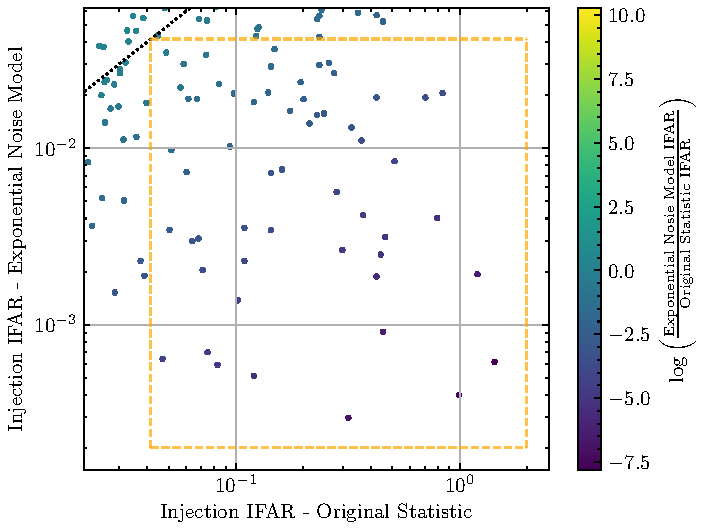
\includegraphics[width=1\textwidth]{images/5_pycbclive/plots/fits_only_ifar_vs_ifar_bottom_left_region.pdf}
    \caption{The inverse false-alarm rate (IFAR) values recorded for each injection that was seen by both the PyCBC Live search that includes the exponential noise model in the ranking statistic and the PyCBC Live search using the same ranking statistic used in the third observing run. Each point represents an injection from the injection set, with the x-axis showing the IFAR recorded using the original ranking statistic and the y-axis showing the IFAR recorded using the exponential noise model ranking statistic. The color bar indicates the logarithmic difference in IFAR between the two searches, with positive values (yellow) indicating better performance when including the exponential noise model in the statistic and negative values (purple) indicating a better performance with the original statistic. The dashed line at y=x represents equal IFAR values for both searches. This figure is zooms in on the yellow dashed box shown in figure~\ref{5:fig:ifar-ifar-fits-only-regions}.}
    \label{5:fig:bottom-left-region}
\end{figure}
%
The original IFAR values of the injections found in this region range from $0.02 - 2.5$ years and the new IFAR values range from $0.0015 - 0.0625$ years, all these injections are found below the $y = x$ diagonal line, indicating a lower IFAR found for the injections with the new ranking statistic. 
%
\begin{figure}
    \centering
    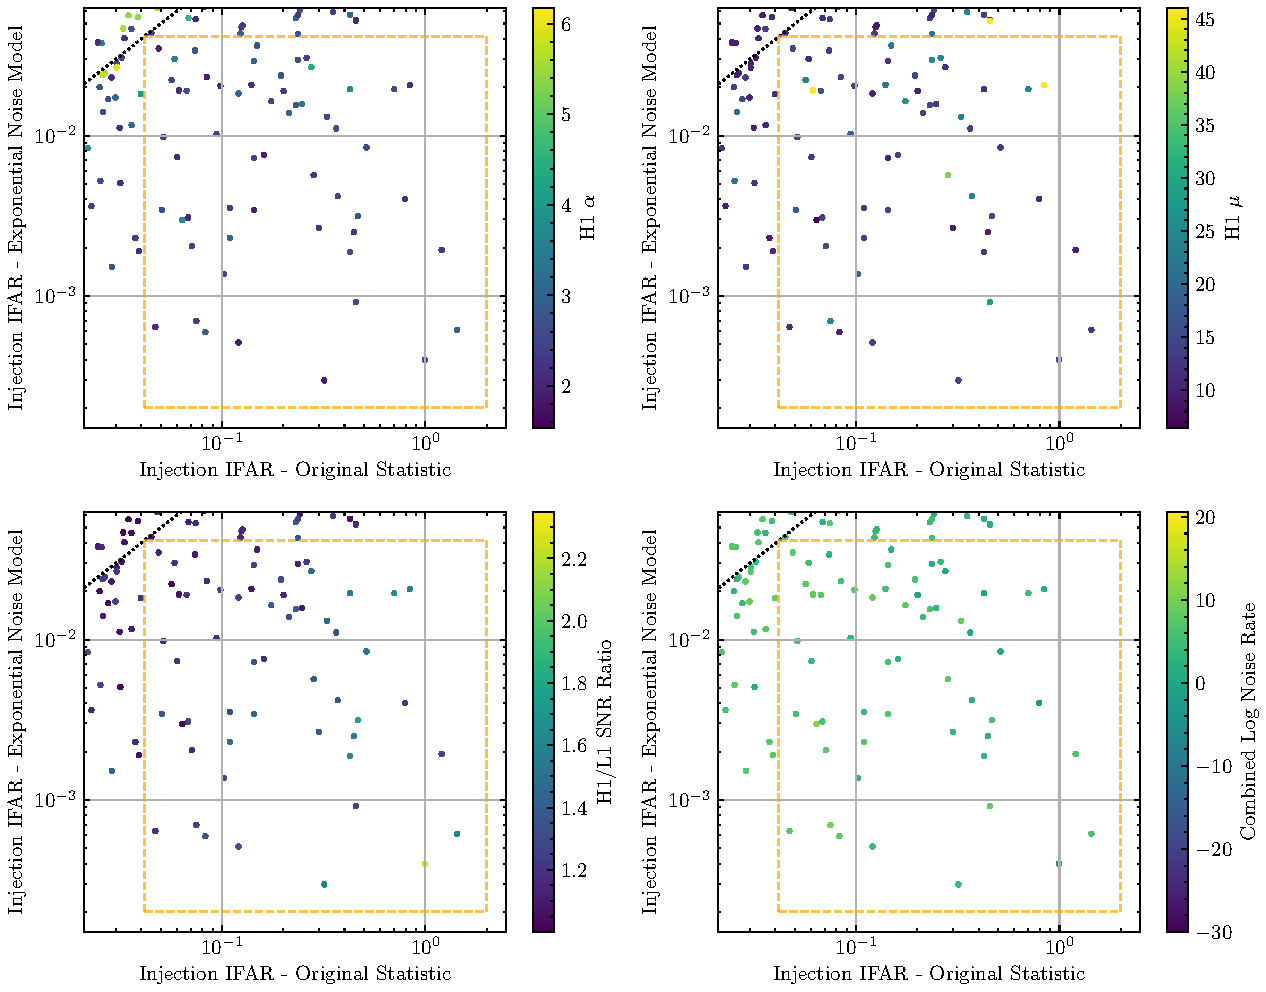
\includegraphics[width=1\textwidth]{images/5_pycbclive/plots/fits_only_ifar_vs_ifar_bottom_left_region_subplots.pdf}
    \caption{The inverse false-alarm rate (IFAR) values recorded for each injection that was seen by both the PyCBC Live search that includes the exponential noise model in the ranking statistic and the PyCBC Live search using the same ranking statistic used in the third observing run. Each point represents an injection from the injection set, with the x-axis showing the IFAR recorded using the original ranking statistic and the y-axis showing the IFAR recorded using the exponential noise model ranking statistic. The top left plot is coloured by the LIGO-Hanford trigger template's exponential fit factor, $\alpha$. The top right plot is coloured by the LIGO-Hanford trigger template's count of triggers found above $\hat{\rho}_{threshold} = 6.0$, $\mu$. The bottom left plot is coloured by the SNR ratio of the two detector $\hat{\rho}$, chosen such that the SNR ratio is always greater than $1$. The bottom right plot is coloured by the combined ($\log$) noise rate~\ref{5:eqn:comb-log-noise-rate}.}
    \label{5:fig:bottom-left-subplots}
\end{figure}
%
Figure~\ref{5:fig:bottom-left-subplots} highlights four different parameters we can investigate to understand why these injections have been down-ranked. Injections that are found further from the diagonal $y = x$ line have been down-ranked more significantly when using the exponential noise model in the ranking statistic. The 2 figures on the top row of figure~\ref{5:fig:bottom-left-subplots} show H1 $\alpha$ and H1 $\mu$ of the injections which represent the contribution to the ranking statistic from the exponential noise model. The majority of the injections have been found with a high noise rate, indicated by low $\alpha$ and high $\mu$ values but there is no correlation between these values and the distance from the diagonal line.

The bottom right figure shows the combined log noise event rate density for the injections and again, there is no clear correlation between distance from the diagonal and noise rate value, the majority of injections have a high noise rate but some templates which have been heavily down-ranked have low noise rates relative to other injections in this region.

The bottom left figure shows the ratio of the two detector $\hat{\rho}$ values identified in the search using the new statistic, calculated such that the ratio is always greater than $1$. This figure shows that injections that have been most significantly down-ranked when using the new statistic have higher SNR ratios, this is caused by the noise rate contributions to the ranking statistic described in section~\ref{5:sec:comparing-statistic-construction} and how the original statistic maximises the squared sum of the detector $\hat{\rho}$ values in the noise rate calculation and the new statistic takes a linear sum of $\hat{\rho}$ with a weighting based on historical noise rate of the trigger template. Therefore, in the new statistic search a low $\hat{\rho}$ in one detector can no longer be compensated for by a much larger $\hat{\rho}$ in the other detector, leading to a decrease in the significance of the injections. This is a consequence of the ranking statistic formulation.

\subsection{\label{5:sec:top-right-region}Down-ranked highly significant injections}

The region indicated in the top right of figure~\ref{5:fig:ifar-ifar-fits-only-regions} by a dashed red box contains injections that were found with the maximum IFAR value with the original ranking statistic but have now been down-ranked by including the exponential noise rate model in the ranking statistic. These injections are still found with a high significance in the new statistic. This region contains $24$ injections, which we can split into two groups for investigation: $12$ injections found with the same trigger in both searches and $12$ injections found with different triggers in both searches. 

% Same Triggers
When an injection is found with the same trigger across both searches we can dismiss any changes in $\hat{\rho}$ being the cause for an IFAR drop. We can analyse these injections to understand whether these injections were down-ranked due to high noise rate templates being responsible for the triggers or if the construction of the ranking statistic has changed their significance.

For each injection found with the same trigger in both searches, table~\ref{5:tab:top-right-same-trigs-fits} shows the individual detector $\hat{\rho}$, the template fit parameters $\alpha$ and $\mu$, the single detector noise event rate density, r$_n$, the combined noise event rate density,$p^{N}(\Vec{\theta})$ , the signal event rate density, $p^{S}(\Vec{\theta})$, and finally the ranking statistic value that these injections were found with using the new ranking statistic.
%
\begin{table}[ht]
    \centering
    \small
    \setlength{\tabcolsep}{4pt}
    \rowcolors{2}{white}{lightgray}
    \begin{tabular}{lccccccccccc}
        \toprule
        & \multicolumn{4}{c}{\textbf{H1}} & \multicolumn{4}{c}{\textbf{L1}} \\
        \cmidrule(lr){2-5} \cmidrule(lr){6-9}
        \textbf{Index} & \textbf{$\hat{\rho}$} & \textbf{$\alpha$} & \textbf{$\mu$} & \textbf{$\log r_n$} & \textbf{$\hat{\rho}$} & \textbf{$\alpha$} & \textbf{$\mu$} & \textbf{$\log r_n$} & \textbf{$\log p^{N}(\Vec{\theta})$} & \textbf{$\log p^{S}(\Vec{\theta})$} & \textbf{Rank. Stat.} \\
        \midrule
        8015 & 8.53 & 2.60 & 24.5 & -2.42 & 9.35 & 2.75 & 22.5 & -5.07 & -11.22 & 0.55 & 11.77 \\
        8026 & 9.31 & 2.37 & 9.4 & -4.74 & 8.88 & 2.52 & 14.4 & -3.67 & -12.14 & -0.91 & 11.23 \\
        8110 & 8.99 & 2.37 & 9.4 & -3.97 & 10.30 & 2.52 & 14.4 & -7.26 & -14.96 & -4.78 & 10.18 \\
        9222 & 10.09 & 2.78 & 15.0 & -7.63 & 9.11 & 2.63 & 23.0 & -4.07 & -15.44 & -3.04 & 12.40 \\
        9365 & 7.34 & 2.57 & 24.0 & 0.68 & 10.88 & 2.28 & 29.0 & -6.94 & -9.99 & 0.14 & 10.13 \\
        9777 & 8.33 & 2.57 & 33.75 & -1.51 & 9.30 & 2.78 & 34.25 & -4.63 & -9.86 & 1.91 & 11.77 \\
        10105 & 9.23 & 2.01 & 13.67 & -3.18 & 8.89 & 2.95 & 20.0 & -4.46 & -11.37 & -0.31 & 11.06 \\
        10251 & 9.52 & 2.37 & 9.4 & -5.23 & 10.26 & 2.52 & 14.4 & -7.17 & -16.14 & -10.22 & 5.92 \\
        10979 & 8.31 & 2.01 & 13.67 & -1.33 & 10.23 & 2.95 & 20.0 & -8.41 & -13.47 & -2.02 & 11.45 \\
        11386 & 12.34 & 2.37 & 9.4 & -11.91 & 6.47 & 2.52 & 14.4 & 2.41 & -13.22 & -5.02 & 8.20 \\
        11608 & 9.93 & 1.93 & 14.5 & -4.24 & 7.68 & 2.83 & 23.75 & -0.56 & -8.52 & 1.07 & 9.59 \\
        13845 & 8.40 & 2.37 & 9.4 & -2.57 & 10.37 & 2.52 & 14.4 & -7.44 & -13.74 & -1.53 & 12.21 \\
        \bottomrule
    \end{tabular}
    \caption{Properties of preferred triggers detected by both the LIGO-Hanford (H1) and LIGO-Livingston (L1) detectors for injections indicated by index number in the injection set. The table shows the new signal-to-noise ratio ($\hat{\rho}$), the exponential fit factor ($\alpha$), the number of triggers above the threshold ($\mu$), and the single detector ($\log$) noise rate ($\log r_n$) for the preferred trigger found by both detectors for each injection. The final columns provide the combined ($\log$) noise rate ($\log p^{N}(\Vec{\theta})$), the ($\log$) signal rate ($\log p^{S}(\Vec{\theta})$), and the ranking statistic value calculated using the ranking statistic including the exponential noise model.}
    \label{5:tab:top-right-same-trigs-fits}
\end{table}
%

% MAYBE REPLACE THIS WITH INJECTION 11608

To demonstrate how the addition of the exponential noise model can cause the down-ranking of an injection we pick injection $11608$ which had the most significant drop, from maximum IFAR in the old statistic to an IFAR of $209.55$ years when found with the new statistic. We display the ranking statistic components for both searches in tables~\ref{5:tab:11608-new-stat} and ~\ref{5:tab:11608-old-stat}.
%
\begin{table}[ht]
    \centering
    \setlength{\tabcolsep}{4pt}
    \begin{minipage}{0.48\textwidth}
        \centering
        \rowcolors{2}{white}{lightgray}
        \begin{adjustbox}{minipage=\linewidth-0cm, margin=0.5cm 0cm 0cm 0cm}
        \begin{tabular}{lcc}
            \toprule
            \textbf{Index = 11608} & \textbf{New Trigger} \\
            \midrule
            $\log p^{N}$  & -8.52 \\
            $\log p^{S}$ & 1.07 \\
            $R_{new}$ & 9.59 \\
            IFAR & 209.55 \\
            \bottomrule
        \end{tabular}
        \end{adjustbox}
        \caption{}
        \label{5:tab:11608-new-stat}
    \end{minipage}
    \hfill
    \begin{minipage}{0.48\textwidth}
        \centering
        \rowcolors{2}{white}{lightgray}
        \begin{tabular}{lcc}
            \toprule
            \textbf{Index = 11608} & \textbf{Original Trigger}\\
            \midrule
            $\rho_{H1,new}^2 + \rho_{L1,new}^2$   & 157.59 \\
            $\log p^{S}$ & 1.07 \\
            $R_{new}$ & 12.60 \\
            IFAR & 30174.69 \\
            \bottomrule
        \end{tabular}
        \caption{}
        \label{5:tab:11608-old-stat}
    \end{minipage}
\end{table}
%
It is important to remember that we cannot directly compare ranking statistic values between the searches, the only values we can compare are the signal rate which is the same for both searches due to this injection being found with the same trigger in both, and the IFAR.

Looking at table~\ref{5:tab:top-right-same-trigs-fits} for injection $11608$ it has low $\alpha$ values of $1.93$ and $2.83$ and therefore is being heavily down-ranked by the template fits, these amount to the highest noise rate in the table of $-8.52$. This injection has a signal rate of $1.07$ which is low, the original statistic initially assigned such a large significance to this injection due to the high quadrature sum of the new SNRs heavily outweighing the low signal rate in the ranking statistic calculation (equation~\ref{5:eqn:original-statistic}) whereas the new statistic placed less significance on the $\hat{\rho}$ from both detectors for this injection, with an equal contribution from both the signal and noise rate (equation~\ref{5:eqn:new-statistic}). While the exponential noise model has down-ranked the significance of this injection, it has still been found with a very high IFAR.

% Different Triggers
When an injection has been found with a different trigger by the new ranking statistic and has still been down-ranked with a lower significance it indicates that the original trigger found by the original statistic would have performed even worse than the new trigger. In section~\ref{5:sec:diff-triggers} we have discussed why different triggers are chosen by the new statistic and we can further demonstrate these using the injections in this region that have been found with a different trigger in the new ranking statistic search. We create the same table for the injections found with different template ids, table~\ref{5:tab:top-right-diff-temp-fits}.
%
\begin{table}[ht]
    \centering
    \small
    \setlength{\tabcolsep}{4pt}
    \rowcolors{2}{white}{lightgray}
    \begin{tabular}{lccccccccccc}
        \toprule
        & \multicolumn{4}{c}{\textbf{H1}} & \multicolumn{4}{c}{\textbf{L1}} \\
        \cmidrule(lr){2-5} \cmidrule(lr){6-9}
        \textbf{Index} & \textbf{$\hat{\rho}$} & \textbf{$\alpha$} & \textbf{$\mu$} & \textbf{$\log r_n$} & \textbf{$\hat{\rho}$} & \textbf{$\alpha$} & \textbf{$\mu$} & \textbf{$\log r_n$} & \textbf{$\log p^{N}(\Vec{\theta})$} & \textbf{$\log p^{S}(\Vec{\theta})$} & \textbf{Rank. Stat.} \\
        \midrule
        8466 & 13.50 & 2.78 & 13.00 & -17.27 & 6.58 & 3.01 & 17.50 & 2.21 & -18.79 & -15.67 & 3.12 \\
        8776 & 6.06 & 2.39 & 25.33 & 3.96 & 12.48 & 2.62 & 26.67 & -12.74 & -12.51 & -0.22 & 12.29 \\
        9040 & 6.20 & 1.93 & 14.50 & 2.95 & 11.01 & 2.83 & 23.75 & -9.99 & -10.77 & -1.30 & 9.47 \\
        9338 & 10.78 & 2.68 & 8.73 & -9.66 & 7.16 & 2.08 & 10.96 & 0.70 & -12.69 & -2.74 & 9.95 \\
        9819 & 7.00 & 1.93 & 14.50 & 1.41 & 11.32 & 2.83 & 23.75 & -10.87 & -13.19 & -1.25 & 11.94 \\
        9859 & 10.39 & 2.58 & 12.86 & -7.83 & 6.61 & 3.69 & 14.57 & 1.74 & -9.81 & -4.62 & 5.19 \\
        10071 & 6.65 & 2.09 & 13.43 & 1.97 & 14.53 & 3.03 & 20.71 & -21.69 & -23.45 & -16.34 & 7.11 \\
        10101 & 10.99 & 2.52 & 18.84 & -8.72 & 7.65 & 3.87 & 17.00 & -2.21 & -14.66 & -6.69 & 7.97 \\
        10134 & 6.55 & 2.60 & 24.50 & 2.72 & 8.76 & 2.75 & 22.50 & -3.46 & -4.47 & 0.09 & 4.56 \\
        10297 & 10.59 & 2.58 & 12.86 & -8.35 & 7.96 & 3.69 & 14.57 & -3.27 & -5.35 & -5.53 & -0.18 \\
        10788 & 9.28 & 2.58 & 12.86 & -4.95 & 8.38 & 3.69 & 14.57 & -4.79 & -13.47 & -0.64 & 12.83 \\
        11505 & 10.78 & 2.78 & 13.00 & -9.71 & 6.67 & 3.01 & 17.50 & 1.95 & -11.48 & -5.97 & 5.51 \\
        \bottomrule
    \end{tabular}
    \caption{Properties of preferred triggers detected by both the LIGO-Hanford (H1) and LIGO-Livingston (L1) detectors for injections indicated by index number in the injection set. The table shows the new signal-to-noise ratio ($\hat{\rho}$), the exponential fit factor ($\alpha$), the number of triggers above the threshold ($\mu$), and the single detector ($\log$) noise rate ($\log r_n$) for the preferred trigger found by both detectors for each injection. The final columns provide the combined ($\log$) noise rate ($\log p^{N}$), the ($\log$) signal rate ($\log p^{S}$), and the ranking statistic calculated using the ranking statistic including the exponential noise model.}
    \label{5:tab:top-right-diff-temp-fits}
\end{table}
%
These injections have very poor fit parameter values with low $\alpha$ values (especially in H1) and high $\mu$ values. One thing that is very clear, especially when compared to the same trigger table, is that these injections were all found with substantial SNR ratios. These injections and their SNR ratios can be seen in figure~\ref{5:fig:ifar-ifar-snr-ratio} and this is a clear demonstration of how high SNR ratio triggers are favoured in the old statistic and are not in the new statistic. Overall most injections have been found with high combined detector noise rates and the signal rates aren't large enough to compensate. This region demonstrates that while injections may be down-ranked using the new ranking statistic we are still achieving an overall increase in sensitivity in this IFAR region (figure~\ref{5:fig:vt-ratio-fits-only}) and we understand the causes of the down-ranking of these highly significant injections.


\subsection{\label{5:sec:middle-region}Down-ranked marginal injections}

The injections found in the blue dashed box in the middle of figure~\ref{5:fig:ifar-ifar-fits-only-regions} are injections which have been found with IFAR above ${\sim}1$ year with the original ranking statistic but have been down-ranked by the new ranking statistic. An IFAR of $1$ year is a conservative threshold that distinguishes \gwadj events as being real or fake, the sensitive ratio plot (figure~\ref{5:fig:vt-ratio-fits-only}) highlights the sensitivity increase at this IFAR threshold as being $43\%$. These are the few injections in this region that have been down-ranked and so we want to understand what has caused this down-ranking. This region only contains $3$ injections and therefore we can investigate each injection individually to understand the cause of their down-ranking.

We can look at the numerical values associated with each injection, this is shown in table~\ref{5:tab:bottom-right-rank-stat}.
%
\begin{landscape}
\begin{table}[tb]
    \centering
    \small
    \setlength{\tabcolsep}{5pt}
    \rowcolors{2}{white}{lightgray}
    \begin{tabular}{lcccccccccccccc}
        \toprule
        & \multicolumn{4}{c}{\textbf{H1}} & \multicolumn{4}{c}{\textbf{L1}} & \multicolumn{3}{c}{\textbf{New}} & \multicolumn{3}{c}{\textbf{Old}} \\
        \cmidrule(lr){2-5} \cmidrule(lr){6-9} \cmidrule(lr){10-12} \cmidrule(lr){13-15}
        \textbf{Index} & \textbf{$\hat{\rho}$} & \textbf{$\alpha$} & \textbf{$\mu$} & \textbf{$\log r_n$} & \textbf{$\hat{\rho}$} & \textbf{$\alpha$} & \textbf{$\mu$} & \textbf{$\log r_n$} & \textbf{$\log p^{N}$} & \textbf{$\log p^{S}$} & \textbf{IFAR} & \textbf{$\hat{\rho}_{H1}^{2} + \hat{\rho}_{L1}^{2}$} & \textbf{$\log p^{S}$} & \textbf{IFAR} \\
        \midrule
        8313  & 5.87 & 2.39 & 15.50 & 5.33 & 12.21 & 3.28 & 19.75 & -16.20 & -14.60 & -15.17 & 0.57 & 183.43 & -15.17 & 40.18 \\
        
        10256 & 9.57 & 2.71 & 16.16 & -5.92 & 8.04 & 3.77 & 19.30 & 8.95 & -0.69 & -1.65 & 0.35 & 119.74 & -1.65 & 1.24 \\
        
        10995 & 8.73 & 2.32 & 10.00 & -2.05 & 10.07 & 1.44 & 18.21 & -1.26 & -7.04 & -8.38 & 0.28 & 151.36 & -8.38 & 3.06 \\
        \bottomrule
    \end{tabular}
    \caption{Properties of preferred triggers detected by both the LIGO-Hanford (H1) and LIGO-Livingston (L1) detectors for injections indicated by index number in the injection set. The table shows the new signal-to-noise ratio ($\hat{\rho}$), the exponential fit factor ($\alpha$), the number of triggers above the threshold ($\mu$), and the single detector ($\log$) noise rate ($\log r_n$) for the preferred trigger found by both detectors for each injection. The `New' columns provide the combined ($\log$) noise rate ($\log p^{N}$), the ($\log$) signal rate ($\log p^{S}$), and the inverse false-alarm rate (IFAR) calculated using the ranking statistic including the exponential noise model. The `Old' columns provide the squared sum of the two detector $\hat{\rho}$s, the ($\log$) signal rate ($\log p^{S}$), and the IFAR values calculated using the ranking statistic used by the PyCBC Live search during the third observing run.}
    \label{5:tab:bottom-right-rank-stat}
\end{table}
\end{landscape}
%
All three of these injections have been found with the same trigger in both searches and demonstrate a few different cases for injection down-ranking. Injection $8313$ was found with the same trigger in both searches and while the new statistic's combined noise rate is very low it isn't enough to overcome the very low signal rate whereas the original statistic placed more weight on the very high L1 $\hat{\rho}$ which has compensated for the relatively low H1 $\hat{\rho}$. This is another case where the SNR ratio has a big impact on the significance of recovered events in the original statistic search. Injection $10256$ was originally found with an IFAR of $1.24$ and has been down-ranked to an IFAR of $0.35$. The L1 noise rate is very high, contributing to a large combined noise rate which, when matched with the signal rate has not produced a very significant ranking statistic value. Finally, injection $10955$ is seen with decent $\hat{\rho}$ in both detectors but the $\alpha$ values are poor, especially in L1. This produces a high combined log noise rate which the signal rate couldn't overcome. 

\section{\label{5:sec:mdc-test}Testing using the full template bank}

To test the implementation of the new additions to the ranking statistic we ran the PyCBC Live search in an `offline' mode where the PyCBC Live search operates how it will for the real low-latency search but all the data is available before the search begins and there is no need to wait for the next analysis segment. This allows the PyCBC Live search to process the data as fast as possible and when using the PyCBC-BBH template bank we could process one week of \gwadj data in as little as $1$ day.

The PyCBC-BBH template bank contains ${\sim}15,000$ templates whereas the template bank used by the PyCBC Live search during the fourth observing run has over $700,000$ templates. Individual users are limited to the amount of memory that can be requested when to perform generating the template bank and so the changes could not be tested using the full template bank during development. To fully test these changes we must use the full template bank and a live dataset which simulates exactly how the real search will operate.

The \gwadj mock data challenge (MDC) replays data from the third observing run with a known set of injections and streams it to the same data infrastructure which streams live data from the \gwadj detectors. This allows the full simulation of the low-latency \gwadj search and unlocks the ability to test changes to the \gwadj low-latency search pipelines even when the \gwadj detectors are not operating, either between observing runs, during maintenance downtime or when the detector's are not working correctly.

We were able to test our changes to the PyCBC Live ranking statistic on the PyCBC Live MDC computational resources, allowing the new ranking statistic to be run a low-latency environment with live streamed data to test for any latency introduced into the search by the new ranking statistic components. The computational resources assigned to the PyCBC Live MDC search are equal to those being used in the PyCBC Live search during the fourth observing run and therefore we do not encounter the previously mentioned memory allocation limitations and related issues.

To test the ranking statistic changes we created static template fits for all templates in the full template bank for a week of data and ran the search on the proceeding weeks during the test. The template fits were not updated during this test and the purpose of the test was not to measure sensitivity improvements but to test for bugs in implementation and if the additional ranking statistic components introduce any lag to the search. During this test we identified a number of bugs which were introducing major lag to the search, after fixing the bugs there is no latency difference between the configuration used during the third observing run and the PyCBC Live search including the new ranking statistic components. Figure~\ref{5:fig:mdc_results} shows the IFAR for \gwadj candidates identified by both the original ranking statistic and the exponential noise model ranking statistic for a single day during the MDC test.
%
\begin{figure}
    \centering
    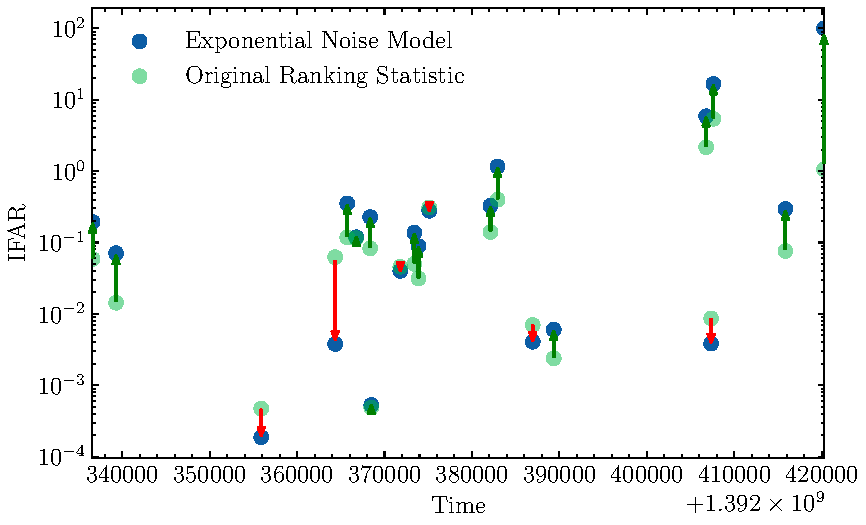
\includegraphics[width=1.0\linewidth]{images/5_pycbclive/plots/mdc_ifar_candidates.pdf}
    \caption{\Gwadj candidates jointly seen by the PyCBC Live full bandwidth Mock Data Challenge (MDC) searches using the original PyCBC Live third observing run ranking statistic (Original Ranking Statistic, green circles) and the PyCBC Live ranking statistic including the exponential noise noise (Exponential Noise Model, blue circles). Events which have been seen with an increased inverse false-alarm rate with the exponential noise model ranking statistic have a green arrow between the original search's circle and the exponential noise model's circle, events seen with a decreased inverse false-alarm rate have a red arrow.}
    \label{5:fig:mdc_results}
\end{figure}
%





\section{\label{5:sec:conclusion}Conclusion}

We have demonstrated that two ranking statistic components taken from the PyCBC Offline search's ranking statistic can be adapted and used in the PyCBC Live search's ranking statistic to improve the overall sensitivity of the PyCBC Live search for \gws. We have implemented the new ranking statistic additions, PSD variation and an exponential noise model, into the PyCBC Live ranking statistic and searched through $1$ week of \gwadj data containing thousands of \gwadj injections with a PyCBC Live search using the original ranking statistic used by PyCBC Live during the third observing run and another PyCBC Live search using a ranking statistic that includes PSD variation and the exponential noise model and compared the false-alarm rates of the injections found by both searches to measure the increase in sensitivity from including the new additions to the ranking statistic. 

We measure an overall increase in sensitivity when both PSD variation and the exponential noise model are included in the ranking statistic however, we measure a greater increase in sensitivity when we do \textbf{not} include PSD variation in the ranking statistic. We also investigate a decrease in sensitivity around a false-alarm rate of $2$ per month by identifying the changes the exponential noise model has made to the ranking statistic to cause the down-ranking of the injections originally found with this false-alarm rate.

We have tested the changes to the PyCBC Live search using the smaller PyCBC-BBH template bank and the complete PyCBC Live template bank being currently used in the fourth observing run and we highlight the difficulty of increasing the complexity of the low-latency search pipeline ranking statistic where changes have the potential to introduce latency to the search pipeline, delaying the dissemination of search results and how the new additions to ranking statistic have not increased the analysis latency of the PyCBC Live search.

The new additions to the PyCBC Live ranking statistic are currently being tested in completeness alongside PyCBC Live infrastructure changes to allow template fit statistics to update weekly based on the previous week's triggers to adapt to changing template noise distributions. The new PyCBC Live ranking statistic will also include data quality information from \texttt{iDQ} and will be run on the second half of the fourth observing run.


%%%%%%%%%%%%%%%%%%%%%%%%%%%%%%%%%%%%%%%%%%%%%%%


% \section*{Appendix}
% \section{\label{5:sec:diff-start-times}How do changes to the search PSD affect the search results?}

% UNCHANGED

% While investigating these regions we discovered a very important contribution to the IFAR vs IFAR distribution that we hadn't intended to include in our injection sets. 

% To take a step back to explain how this problem was introduced into our data and describe how the initial searches were performed. We have two searches: one with the old statistic, one with the new statistic (including any new components). One of the new components is the template fitting statistic and this required that an additional week of search had to be performed using the old statistic, a week prior to the actual search. Therefore for simplicity we ran the old statistic live search over two weeks with no interruptions and the new statistic live search simply over the second week only, after creating the template fitting files.

% The old statistic search began at a GPS time of $1262390400$, with the second week beginning at $1262995020$ so the new statistic search began at this time. The problem is that the difference between the week 1 and week 2 start time ($604,620$) is not divisible by $8$, which is our stride time in live. This means that when the old statistic search is crossing the boundary between week 1 and week 2 it will start week 2 on the stride time $1262995024$ which is four seconds after the offical beginning of week 2.

% An easy to see problem is that the old statistic search will have had more initial time to bed in the search, so it had knowledge of the $256$ seconds prior to the start of week 2, we account for this and exclude $256$ seconds of data from the start of both searches. This should prevent the old statistic search from reporting seeing more injections than the new statistic.

% A bigger problem is that the live searches are analysing different data as they are searching, there is always going to be a $4$ second difference in the data being analysed at any one time. While both searches will search through the same data (except the old statistic will miss the final $4$ seconds of week 2) the PSD for the $256$ seconds of data being analysed can be different in every stride. All the injections have the potential to be seen with a different SNR due to different noise in the data that is being analysed, therefore while the injections might've been seen with the same template, it was not seen with the same trigger which will change the significance of our injections.

% This was discovered when we were seeing different SNR and $\chi^{2}$ values for injections with identical trigger templates and times. Aside from computing issues, our searches should be identical and if they are searching the same data with the same template they should always recover the same values from matched filtering, evidently they weren't due to this mismatch in data.

% To solve this problem we re-ran the new statistic search but with the start time being equal to the start time of the old statistic search, $1262995024$. With this re-run search we can re-plot figure~ADD now that the same data is being analysed in every stride by both searches, this IFAR vs IFAR plot can be seen in figure~\ref{5:fig:ifar-ifar-fits-only-0s},
% %
% \begin{figure}
%        \centering
%     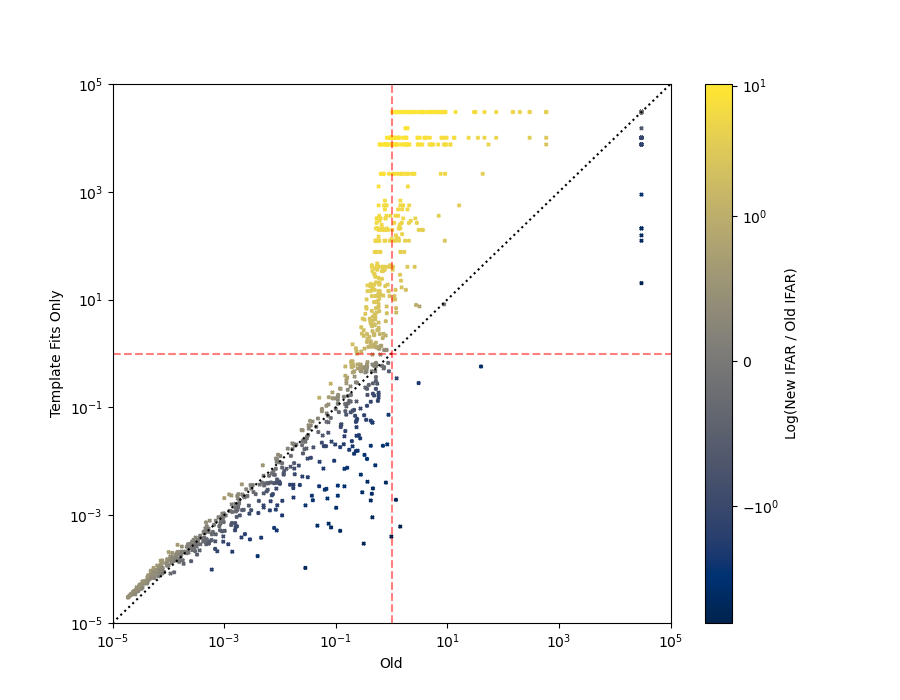
\includegraphics[width=1.2\textwidth]{images/5_pycbclive/plots/fits_only_0s_ifar_vs_ifar_log_ifar_diff.png}
%     \caption{}
%     \label{5:fig:ifar-ifar-fits-only-0s}
% \end{figure}
% %
% and you can see this correction has reduced the spread in the distribution of injections dramatically and is accounting for a lot of the random nature the distribution had in the lower-left quadrant. With this new IFAR vs IFAR plot we are able to re-identify the three regions which will be focus the rest of this section discussing, these regions are highlighted in figure~\ref{5:fig:ifar-ifar-fits-only-0s}.
% %
% \begin{figure}
%     \centering  
%     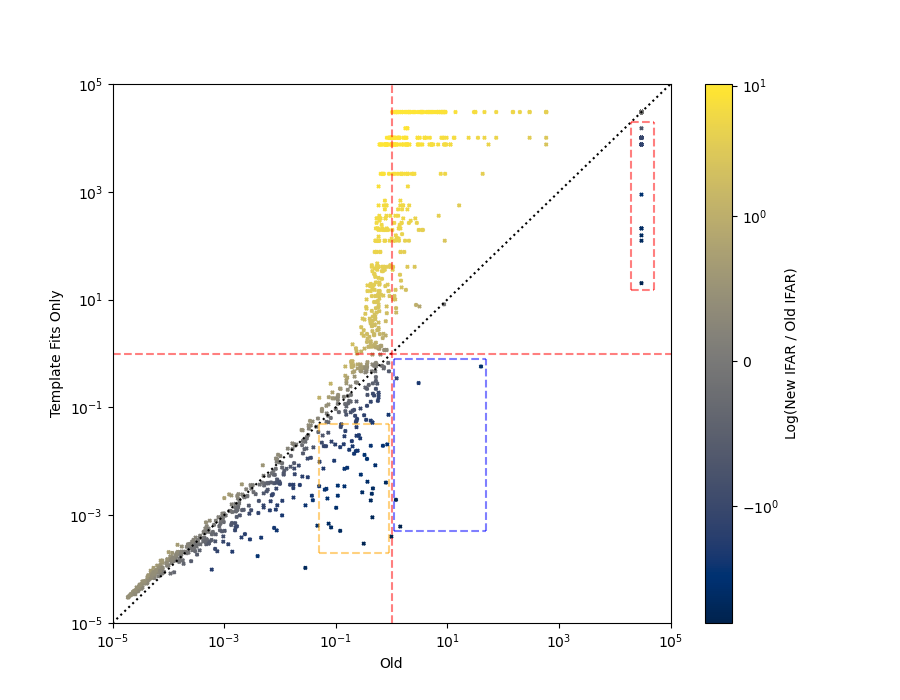
\includegraphics[width=1.2\textwidth]{images/5_pycbclive/plots/fits_only_0s_ifar_vs_ifar_regions.png}
%     \caption{}
%     \label{5:fig:ifar-ifar-fits-only-0s-regions}
% \end{figure}
% %
% \begin{figure}
%     \centering
%     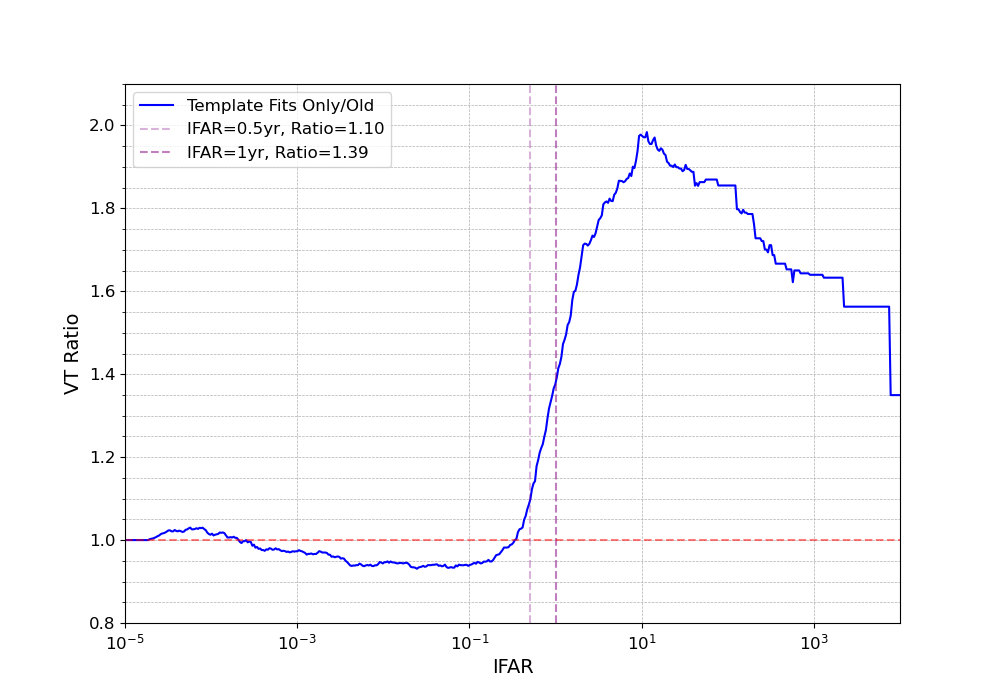
\includegraphics[width=1\textwidth]{images/5_pycbclive/plots/fits_only_0s_vt_ratio.png}
%     \caption{}
%     \label{5:fig:sensitivity-fits-only-0s}
% \end{figure}
% %
% Of the $1275$ jointly observed injections: $704$ are seen with a higher IFAR when including template fits, $309$ with a lower IFAR and, $262$ with the same IFAR. This isn't a complete picture, we don't want to see just an increase in the number of injections with a higher IFAR but higher IFAR values for all out injections. To see this we can look at the VT ratio sensitivity plot, shown in figure~\ref{5:fig:sensitivity-fits-only-0s}.

